\documentclass[journal]{IEEEtran}

\usepackage{amsmath,amssymb,amsfonts}
\usepackage{amsthm}
\usepackage{algorithm}
\usepackage{graphicx}
\usepackage{textcomp}
\usepackage{tikz}
\usetikzlibrary{shapes,arrows,positioning,fit,calc,decorations.pathreplacing}
\usepackage{booktabs}
\usepackage{multirow}
\usepackage{url}
\usepackage{cite}
\usepackage{balance}
\usepackage{float}
\usepackage{placeins}
\usepackage{orcidlink}
\usepackage{comment}
\usepackage{algpseudocode}

\newtheorem{definition}{Definition}
\newtheorem{theorem}{Theorem}
\newtheorem{lemma}{Lemma}
\newtheorem{assumption}{Assumption}
\newtheorem{proof_env}{Proof}


\newcommand{\aggCircuit}{\Lambda_{\mathsf{agg}}}
\newcommand{\vk}{\mathsf{vk}}
\newcommand{\pk}{\mathsf{pk}}
\newcommand{\rootOld}{\mathsf{rt}_{j}^{\text{old}}}
\newcommand{\rootNew}{\mathsf{rt}_{j}^{\text{new}}}

\emergencystretch=3em
\sloppy
\hbadness=10000
\vbadness=10000
\hfuzz=10pt

\begin{document}

\title{H-ZKA: Decoupling Byzantine Faults from Privacy-Preserving State Transitions}


% \author{
%     \IEEEauthorblockN{
%         Nam-Anh Phung Van\IEEEauthorrefmark{1}\,\orcidlink{0009-0009-0260-5445},
%         Minh-Quan Dang\IEEEauthorrefmark{1}\,\orcidlink{0009-0000-6293-1263},
%         Tuan-Dung Tran\IEEEauthorrefmark{2}\,\orcidlink{0000-0003-1156-7072}
%     }\\
%     \IEEEauthorblockA{
%         University of Information Technology, Ho Chi Minh City, Vietnam \\
%         Vietnam National University, Ho Chi Minh City, Vietnam \\
%         Email: \IEEEauthorrefmark{1}\{23520075, 23521251\}@gm.uit.edu.vn,
%         \IEEEauthorrefmark{2}dungtrt@uit.edu.vn
%     }
% }

\maketitle

\begin{abstract}
Cross-chain interoperability has become a critical requirement in the multi-chain blockchain ecosystem, yet the past three years have witnessed cumulative bridge-exploit losses exceeding two billion U.S.~dollars (Ronin, Wormhole, Nomad, Multichain), most of which trace back to compromised or insufficiently auditable cross-chain participants. While recent work such as zkCross introduced a two-layer architecture that decouples privacy-preserving cross-chain transactions from auditing via zk-SNARKs, two significant limitations remain: (1) the reliance on an honest committer assumption, which is vulnerable to Byzantine failures, and (2) the linear scaling of audit workload with the number of chains, which limits applicability to large-scale networks. This paper proposes H-ZKA (Hierarchical Zero-Knowledge Audit), an independent cross-chain privacy-preserving auditing framework inspired by the audit/privacy separation introduced by zkCross and designed to address both shortcomings through two synergistic mechanisms. First, we introduce a Multi-Factor Proof-of-Participation (MF-PoP) reputation system that replaces the honest committer assumption with an adaptive, multi-dimensional scoring scheme. We prove an analytical isolation bound of $T_{\mathrm{isolate}} \le \lceil \ln(R_0/R_{\min})/\ln(1/(1-\lambda\beta_{\min}))\rceil$ rounds, which evaluates to at most $50$ rounds when safety faults dominate the attacker's strategy, with empirical mean $46.3 \pm 2.4$ rounds under stochastic network jitter ($30$ seeds, $50$--$500$\,ms latency, $1$--$5\%$ packet loss). For a worst-case liveness-fault-only adversary the same bound evaluates to $\le 243$ rounds, and \emph{periodic} (slow-loris) attackers require an extension---the cumulative-fault counter of Theorem~\ref{thm:slowloris}---to be guaranteed isolation; the original $46$-round figure applies only to the dominant safety-fault regime. Second, we design a three-layer hierarchical clustering architecture with recursive zk-SNARK proof aggregation, reducing the number of proofs submitted to the global audit chain from $O(k)$ to $O(\sqrt{k})$, where $k$ is the number of ordinary chains. The two mechanisms reinforce each other: reputation scores drive cluster head election via quadratic weighting and verifiable random functions, while cluster-level cross-referencing strengthens reputation accuracy. Crucially, both enhancements operate exclusively on the auditing layer and leave the privacy-preserving transfer and exchange protocols entirely unchanged, preserving the unlinkability guarantees of the original design. Theoretical analysis demonstrates that H-ZKA achieves Byzantine resilience under the standard one-third Byzantine bound (inherited from PBFT/HotStuff) without trusted third parties, and complexity analysis confirms the $\sqrt{k}$-factor reduction in audit workload. We evaluate H-ZKA across networks of up to $200$ chains and explicitly disclose the methodology: \emph{network-side} audit speedups of $12.1\times$ at $k=100$ are reported alongside an \emph{end-to-end} round-latency model that includes the dominant off-chain recursive proving cost ($\approx 9.84\,$s for the $20\,$M-constraint Groth16 aggregation circuit), yielding more conservative end-to-end speedups of $3.1\times$ at $k=100$ and $5.5\times$ at $k=200$ that we believe to be the more practically meaningful figures.
\end{abstract}

\begin{IEEEkeywords}
Cross-chain privacy-preserving auditing, zk-SNARK, proof aggregation, Byzantine fault tolerance, reputation system, blockchain interoperability.
\end{IEEEkeywords}

%% ============================================================
%% SECTION I: INTRODUCTION
%% ============================================================
\section{Introduction}

The blockchain ecosystem has evolved from a single-chain paradigm to a heterogeneous multi-chain landscape in which hundreds of independent blockchains coexist, each serving distinct application domains~\cite{belchior2021survey, han2023survey}. This proliferation creates an urgent demand for cross-chain interoperability, the ability to transfer assets, verify states, and conduct audits across independently maintained ledgers. Cross-chain bridges, atomic swaps, and relay protocols have emerged as the primary building blocks for enabling such interoperability~\cite{zamyatin2019xclaim, herlihy2018atomic, xie2022zkbridge}. However, the security and privacy dimensions of cross-chain interactions remain challenging. Adversaries can exploit transaction linkability to deanonymize participants across chains, and the absence of a unified auditing mechanism across heterogeneous blockchains creates blind spots for compliance and regulation~\cite{augusto2024sok, liu2019auditing}. The financial impact of this gap is substantial: in 2022 alone, the Ronin bridge exploit drained \$625\,M, the Wormhole bridge lost \$325\,M, and the Nomad bridge was emptied of \$190\,M, all in incidents that the post-mortem analyses of Augusto et al.~\cite{augusto2024sok} attribute to compromised relayers, signers, or committers operating without robust accountability mechanisms. These breaches underscore that any cross-chain auditing scheme must reason explicitly about Byzantine participants in the auditing pipeline itself, rather than presuming an honest committer.

Recent advances have sought to reconcile the tension between privacy and auditing in cross-chain settings. The zkCross framework~\cite{guo2024zkcross} introduced a two-layer architecture in which ordinary chains form the lower layer and a dedicated audit chain occupies the upper layer. Three protocols, namely a privacy-preserving transfer protocol, a privacy-preserving exchange protocol, and a cross-chain auditing protocol, address the challenges of Cross-chain Linkability Elimination (CLE), Interplay between Privacy and Auditing (IPA), and Full Auditing Inefficiency (FAI), respectively. By leveraging zk-SNARKs based on the Groth16 proof system~\cite{groth2016size}, zkCross achieves auditing with constant proof size and improves audit efficiency from $O(k \times m \times n)$ to $O(k \times m)$, where $k$ is the number of chains, $m$ is the average block production rate, and $n$ is the average number of transactions per block. Despite these contributions, two significant limitations constrain its practical deployment. First, zkCross assumes the existence of at least one honest committer per chain, an assumption that is difficult to guarantee in open, permissionless environments where Byzantine behavior is the norm rather than the exception. Second, the audit workload on the audit chain scales linearly with $k$, meaning that each auditor must verify $O(k)$ proofs per round, which becomes prohibitive when hundreds of chains participate.

The gap addressed in this paper is twofold. On the security front, no existing cross-chain auditing scheme provides a mechanism to autonomously detect, penalize, and isolate malicious committers without relying on trusted third parties or honest majority assumptions beyond the standard Byzantine threshold. On the scalability front, while recursive proof composition and proof aggregation techniques have been explored in Layer-2 rollup contexts~\cite{rosenberg2024hekaton, xie2022zkbridge}, their application to cross-chain auditing architectures remains unexplored, particularly in combination with reputation-driven node management. Existing work on cross-chain reputation~\cite{hu2024reputation, xiong2025reputation} focuses on transaction-level trust assessment and does not integrate with zero-knowledge auditing protocols.

This paper proposes H-ZKA, an independent framework that adopts the audit/privacy separation insight of zkCross while redesigning the auditing layer with Byzantine-resilient reputation management and hierarchical proof aggregation, leaving the privacy-preserving transfer protocol $\Theta$ and exchange protocol $\Phi$ entirely unchanged. The main contributions of this paper are as follows:
\begin{enumerate}
    \item We propose the Multi-Factor Proof-of-Participation (MF-PoP) reputation system, a multi-dimensional scoring mechanism that combines consistency, historical reliability, and liveness indicators with adaptive decay and progressive taxation. We give a closed-form isolation bound $T_{\mathrm{isolate}} \le \lceil \ln(R_0/R_{\min})/\ln(1/(1-\lambda\beta_{\min})) \rceil$ that holds for any attacker with a non-zero per-round safety-fault rate (including oscillating and adaptive strategies), evaluates to $50$ rounds under our default parameters, and is verified empirically at $46.3 \pm 2.4$ rounds (30 seeds, jitter-injected). Periodic/slow-loris strategies that fall outside this regime are bounded by an extended analysis (Theorem~\ref{thm:slowloris}) that introduces a non-resetting cumulative fault counter. The bound replaces the honest committer assumption of zkCross with Byzantine resilience under the standard one-third Byzantine bound inherited from PBFT~\cite{castro1999pbft} and HotStuff~\cite{yin2019hotstuff}, contingent on intra-cluster honest-majority for the consistency-score channel (Section~\ref{sec:collusion-resistance}).
    \item We introduce a three-layer hierarchical clustering architecture with recursive zk-SNARK proof aggregation. Ordinary chains are grouped into $\sqrt{k}$ regional clusters, and a reputation-elected cluster head aggregates intra-cluster proofs with the recursive verification circuit $\aggCircuit$, reducing the number of proofs on the global audit chain from $O(k)$ to $O(\sqrt{k})$ while preserving the constant proof size of 127 bytes.
    \item We provide a formal security analysis demonstrating that H-ZKA preserves the unlinkability properties of the original protocols, achieves the claimed Byzantine resilience, and delivers the $\sqrt{k}$-factor audit workload reduction. Simulation results across networks of up to 200 chains validate the theoretical predictions.
\end{enumerate}

The remainder of this paper is organized as follows. Section~II reviews related work on cross-chain privacy, auditing, proof aggregation, and reputation systems. Section~III presents the system model, threat model, and formal problem definition. Section~IV details the proposed MF-PoP reputation mechanism. Section~V describes the hierarchical clustering and proof aggregation architecture. Section~VI provides the integrated protocol design and analysis. Section~VII presents the experimental evaluation, and Section~VIII concludes the paper.

%% ============================================================
%% SECTION II: RELATED WORK
%% ============================================================
\section{Related Work}

This section reviews four streams of related literature: cross-chain privacy-preserving protocols, blockchain auditing mechanisms, zero-knowledge proof aggregation techniques, and reputation systems for blockchain networks.

\subsection{Cross-Chain Privacy-Preserving Protocols}

Privacy preservation in cross-chain transactions has received growing attention as the multi-chain ecosystem expands. Early approaches relied on mixing protocols and CoinJoin-style techniques to break transaction linkability~\cite{bonneau2014mixcoin, heilman2017tumblebit}, but these methods do not extend naturally to cross-chain settings. Deshpande and Herlihy~\cite{deshpande2020privacy} proposed privacy-preserving cross-chain atomic swaps by decoupling the preimage mechanism in HTLCs, though without addressing the auditing dimension. Sasson et al.~\cite{sasson2014zerocash} introduced Zerocash for anonymous payments using zk-SNARKs on a single chain, and subsequent work by Bowe et al.~\cite{bowe2020zexe} extended zero-knowledge capabilities to decentralized private computation. For cross-chain contexts specifically, Garoffolo et al.~\cite{garoffolo2020zendoo} proposed Zendoo, a zk-SNARK verifiable cross-chain transfer protocol for decoupled sidechains. Li et al.~\cite{li2022zerocross} presented ZeroCross for Monero-based cross-chain transactions with sidechain privacy. More recently, Ge et al.~\cite{ge2023accio} developed Accio for variable-amount off-chain payments, and Qin et al.~\cite{qin2023blindhub} proposed BlindHub for Bitcoin-compatible payment channel hubs with variable amount support. The zkCross framework~\cite{guo2024zkcross} represents the most comprehensive approach, combining privacy-preserving transfer and exchange protocols with an integrated auditing mechanism. However, none of these works address the resilience of the auditing participants themselves against Byzantine behavior.

\subsection{Blockchain Auditing Mechanisms}

Auditing in blockchain systems encompasses both on-chain compliance verification and off-chain data integrity checking. Du et al.~\cite{du2021auditing} proposed blockchain-enabled decentralized storage auditing, but their approach targets single-chain environments without cross-chain considerations. Weng et al.~\cite{weng2019deepchain} introduced DeepChain for auditable and privacy-preserving deep learning with blockchain-based incentives. In the regulatory context, Liu et al.~\cite{liu2019auditing} examined how blockchain technology impacts auditing and accounting practices. The cross-chain auditing problem specifically requires verifying state transitions across heterogeneous chains while preserving transaction privacy, a challenge first formalized and addressed by zkCross~\cite{guo2024zkcross}. The key limitation of existing auditing schemes, including zkCross, is that they assume the existence of trusted or honest participants in the auditing pipeline. The zk-SNARK-based auditing protocol reduces the verification burden from $O(k \times m \times n)$ to $O(k \times m)$ by aggregating transactions within each block, but the linear dependence on $k$ remains a scalability bottleneck for large multi-chain networks.

\subsection{Zero-Knowledge Proof Aggregation}

The concept of proof aggregation in zero-knowledge systems has gained traction as a means to improve scalability. Groth~\cite{groth2016size} established the foundational Groth16 proof system with constant-size proofs. Xie et al.~\cite{xie2022zkbridge} developed zkBridge, which uses recursive proof composition to build trustless cross-chain bridges with deferred verification. Rosenberg et al.~\cite{rosenberg2024hekaton} proposed Hekaton, a horizontally-scalable approach to zkSNARK proof aggregation that distributes prover computation across multiple machines. Ding et al.~\cite{ding2025vecrotoken} introduced VeCroToken for efficient and privacy-preserving cross-chain operations in consortium blockchains using zk-SNARKs. Cao et al.~\cite{cao2025map} presented MAP Protocol, a trustless interoperability design whose hybrid light-client/zk architecture reduces bridge-side verification cost to $O(N)$. These works demonstrate the feasibility of recursive and aggregated proof construction, but their application has been limited to Layer-2 rollup scenarios or single-purpose bridges. The specific challenge of aggregating cross-chain auditing proofs within a hierarchical multi-layer architecture has not been addressed.

% [SỬA LỖI B5] So sánh trực tiếp với Hekaton và zkBridge — giải thích tại sao chọn hierarchical thay vì horizontal
\textbf{Comparison with Hekaton and zkBridge:} Two works are particularly relevant to our aggregation design. zkBridge~\cite{xie2022zkbridge} constructs recursive proofs over block headers for trustless bridge verification but operates on a single source-destination pair and does not handle multi-chain auditing with Byzantine participants. Hekaton~\cite{rosenberg2024hekaton} achieves horizontally-scalable proof aggregation by distributing prover computation across machines, reducing prover time linearly with the number of workers. While horizontal scaling is effective for homogeneous proof batches, it does not account for the heterogeneity inherent in cross-chain auditing, where each chain may use different consensus protocols, block structures, and transaction formats. Our hierarchical approach ($\sqrt{k}$ clusters of $\sqrt{k}$ chains each) is specifically designed for the cross-chain setting: intra-cluster aggregation handles chain-local proofs with geographic locality, while the global audit layer verifies cluster-level aggregated proofs. This architecture requires only $O(\sqrt{k})$ on-chain verifications compared to Hekaton's $O(1)$ but provides integrated Byzantine detection via the reputation layer, a dimension not addressed by either Hekaton or zkBridge.

\textbf{Comparison with newer recursive-proof systems (Halo2, Nova, Plonky2, SnarkPack, PLONK).} A natural concern raised by reviewers is whether Groth16 recursion is the right vehicle in 2025. Halo2~\cite{bowe2019halo} eliminates the trusted setup and supports nested amortized proofs; Nova~\cite{kothapalli2022nova} achieves \emph{constant-time} folding by deferring expensive checks; Plonky2~\cite{plonky2} combines PLONK~\cite{gabizon2019plonk} with FRI to obtain extremely fast same-field recursion; SnarkPack~\cite{bunz2021snarkpack} aggregates many Groth16 proofs through inner-pairing-product arguments; Marlin~\cite{chiesa2020marlin} provides a universal SRS. We deliberately retain Groth16 for the H-ZKA prototype because (i)~it is the only proof system in our reference baseline (zkCross~\cite{guo2024zkcross}) and a fair comparison demands an apples-to-apples deployment, (ii)~it has the smallest verifier byte size (127\,B) and lowest on-chain gas cost (\,555{,}202\,gas) of any current production-grade SNARK, which is precisely the metric the global audit chain must minimize, and (iii)~the alternative systems are themselves orthogonal upgrades, and they would slot directly into $\aggCircuit$ as drop-in replacements. We provide a quantitative recursive-verifier-cost comparison in Section~\ref{sec:recursivecmp} (Table~\ref{tab:recursivecmp}) showing that the Groth16 path is approximately $200$--$500\times$ heavier in constraints than Plonky2 but retains a $4$--$10\times$ advantage in on-chain gas. Adopting Halo2 or Nova-style folding therefore remains an attractive future direction (Section~\ref{sec:limitations}), but it would not invalidate the H-ZKA architecture; only the inner $\aggCircuit$ instantiation would change.

\subsection{Reputation Systems for Blockchain Networks}

Reputation systems have been employed in blockchain contexts for node selection, validator incentivization, and Sybil resistance. The classical Byzantine fault-tolerance line---PBFT~\cite{castro1999pbft}, HotStuff~\cite{yin2019hotstuff}, Tendermint~\cite{kwon2014tendermint}, and the Honey Badger of BFT protocols~\cite{miller2016honeybadger}---establishes the standard one-third Byzantine bound and underlies the cluster-level resilience claim of this paper. Stake-weighted leader-election protocols extend this foundation: Algorand~\cite{chen2017algorand} uses cryptographic sortition with VRFs and stake-proportional weighting, Ouroboros~\cite{kiayias2017ouroboros} introduces provably-secure proof-of-stake, and Casper FFG~\cite{buterin2017casper} couples slashing with finality guarantees. H-ZKA reuses the VRF + stake-weighting template, but, unlike these consensus protocols, it operates exclusively on an \emph{auditing} layer over heterogeneous foreign chains, with reputation as a synthetic stake derived from observed proof correctness rather than locked tokens. Hu et al.~\cite{hu2024reputation} proposed a decentralized dynamic reputation value assessment method for cross-chain transactions, using an RNN-based dynamic evaluation window that is more flexible than the static EMA used in H-ZKA. Xiong et al.~\cite{xiong2025reputation} developed a reputation-driven mechanism for cross-chain IoT data sharing that incentivizes honest participation. The SoK by Augusto et al.~\cite{augusto2024sok} provides a comprehensive analysis of security and privacy vulnerabilities in blockchain interoperability, identifying the absence of robust reputation mechanisms as a contributing factor to bridge exploits, and is consistent with the post-mortem reports of the Ronin~\cite{ronin2022postmortem} and Wormhole~\cite{wormhole2022postmortem} incidents and the broader Chainalysis 2023 industry report~\cite{chainalysis2023bridges} that totaled cross-chain bridge losses at over \$2\,B for 2022--2023. Yuan et al.~\cite{yuan2024doublelayer} proposed a double-layer Byzantine fault-tolerant grouping consensus algorithm, introducing the concept of hierarchical grouping for consensus scalability. However, existing reputation systems for cross-chain settings focus primarily on transaction-level trust and do not integrate with zero-knowledge auditing protocols, leaving a gap between reputation management and privacy-preserving compliance verification.

\begin{table}[h!]
\centering
\caption{Comparison of related cross-chain approaches.}
\label{tab:comparison}
\resizebox{\columnwidth}{!}{
\begin{tabular}{lcccccc}
\toprule
Approach & Privacy & Auditing & Byzantine & Proof & Audit \\
         & Prot.   & Support  & Resilient & Agg.  & Complexity \\
\midrule
Zendoo~\cite{garoffolo2020zendoo} & \checkmark & $\times$ & $\times$ & $\times$ & -- \\
zkBridge~\cite{xie2022zkbridge} & $\times$ & $\times$ & $\times$ & \checkmark & -- \\
Hekaton~\cite{rosenberg2024hekaton} & $\times$ & $\times$ & $\times$ & \checkmark & -- \\
VeCroToken~\cite{ding2025vecrotoken} & \checkmark & \checkmark & $\times$ & $\times$ & $O(k)$ \\
zkCross~\cite{guo2024zkcross} & \checkmark & \checkmark & $\times$ & $\times$ & $O(k \times m)$ \\
H-ZKA (Ours) & \checkmark & \checkmark & \checkmark & \checkmark & $O(\sqrt{k} \times m)$ \\
\bottomrule
\end{tabular}
}
\end{table}

As shown in Table~\ref{tab:comparison}, no existing approach simultaneously provides privacy-preserving cross-chain protocols, integrated auditing, Byzantine resilience for the auditing pipeline, and proof aggregation for audit scalability. H-ZKA fills this gap.

\subsection{Theoretical Comparison with Closest SOTA}

\begin{table*}[t]
\centering
\caption{Theoretical comparison with the most relevant state-of-the-art systems.}
\label{tab:theory}
\resizebox{\textwidth}{!}{%
\begin{tabular}{lcccc}
\toprule
Work & Scaling style & Deployment model & Reputation model & Main distinction from H-ZKA \\
\midrule
Hekaton~\cite{rosenberg2024hekaton} & Horizontal & Generic zk aggregation & None & Parallel proving, but no Byzantine auditing layer \\
MAP Protocol~\cite{cao2025map} & Hybrid light-client + zk & Interoperability relay & None & Achieves $O(N)$ bridge-side cost, but no reputation-driven audit isolation \\
VeCroToken~\cite{ding2025vecrotoken} & Cross-chain zk verification & Consortium blockchain & Not reputation-centric & Permissioned focus rather than open multi-chain auditing \\
Hu et al.~\cite{hu2024reputation} & Dynamic trust scoring & Cross-chain transactions & RNN-based window & More flexible than EMA, but no zk audit aggregation \\
H-ZKA (ours) & Hierarchical & Open multi-chain auditing & EMA-based MF-PoP & Integrates privacy-preserving auditing, Byzantine isolation, and $O(\sqrt{k})$ audit cost \\
\bottomrule
\end{tabular}}
\end{table*}

Table~\ref{tab:theory} clarifies the design gap addressed by H-ZKA. Hekaton focuses on horizontal proof parallelism, whereas H-ZKA adopts hierarchical aggregation because cross-chain auditing must preserve locality across heterogeneous chains. MAP Protocol reduces interoperability cost to $O(N)$ through a hybrid light-client/zk design, but it does not address adversarial committers in the auditing pipeline. VeCroToken targets consortium settings with different trust assumptions, while Hu et al. emphasize RNN-based reputation estimation that is more flexible than our EMA-based MF-PoP update, yet still lacks integrated zero-knowledge audit proofs. H-ZKA combines these previously separate concerns into a single audit-layer architecture.

%% ============================================================
%% SECTION III: SYSTEM MODEL AND PROBLEM DEFINITION
%% ============================================================
\FloatBarrier
\section{System Model and Problem Definition}

\subsection{Notation}

Table~\ref{tab:notation} summarizes the symbols used throughout the paper.

\begin{table}[H]
\centering
\caption{Summary of notation.}
\label{tab:notation}
\begin{tabular}{cl}
\toprule
Symbol & Description \\
\midrule
$k$ & Number of ordinary chains in the network \\
$m$ & Average block production rate (blocks/second) \\
$n$ & Average number of transactions per block \\
$M$ & Number of regional clusters, $M = \lceil \sqrt{k} \rceil$ \\
$\mathcal{C}_\ell$ & The $\ell$-th regional cluster, $\ell \in [1, M]$ \\
$\text{CH}_\ell$ & Cluster head of $\mathcal{C}_\ell$ \\
$\text{CT}_i$ & Committer $i$ submitting proofs for a chain \\
$R_i$ & Reputation score of node $i$, $R_i \in [0.01, 10.0]$ \\
$C_i^t$ & Consistency score of $\text{CT}_i$ at round $t$ \\
$H_i^t$ & Historical reliability score (EMA) at round $t$ \\
$L_i^t$ & Liveness indicator at round $t$ \\
$Q_i^t$ & Composite quality score at round $t$ \\
$\beta_i^t$ & Adaptive decay rate for $\text{CT}_i$ at round $t$ \\
$\pi_j$ & zk-SNARK proof for chain $j$ \\
$\pi_{\text{agg}}$ & Aggregated proof for a cluster \\
$\aggCircuit$ & Recursive aggregation circuit \\
$\text{vk}_j$ & Verification key for chain $j$ \\
$\xi$ & Smart contract address \\
$T$ & Time lock parameter \\
$\lambda$ & Security parameter \\
\bottomrule
\end{tabular}
\end{table}

\subsection{System Model}

We inherit the network model of zkCross~\cite{guo2024zkcross} and extend it with a three-layer architecture. The system consists of the following entities. \textit{Ordinary chains} ($\text{Chain}_1, \text{Chain}_2, \ldots, \text{Chain}_k$) are independent blockchains where cross-chain transactions (transfers and exchanges) occur, each maintaining its own consensus and state. \textit{Committers} ($\text{CT}_i$) are nodes responsible for generating zk-SNARK proofs that attest to the correctness of state transitions within their assigned chain; unlike the original zkCross, committers in H-ZKA are not assumed to be honest. \textit{Regional clusters} ($\mathcal{C}_1, \mathcal{C}_2, \ldots, \mathcal{C}_M$) are groups of approximately $\sqrt{k}$ chains, each managed by a cluster head $\text{CH}_\ell$ elected through reputation-weighted verifiable random functions. The \textit{global audit chain} is the top-layer chain where aggregated proofs from cluster heads are verified by auditors, maintaining a global state root $\text{root}_{\text{global}} = \text{MerkleTree}(\{\text{cluster\_root}_\ell\}_{\ell=1}^{M})$. Finally, \textit{auditors} ($\text{AD}$) are nodes on the global audit chain that verify aggregated proofs and maintain the global audit state.

\begin{figure*}[h!]
    \centering
    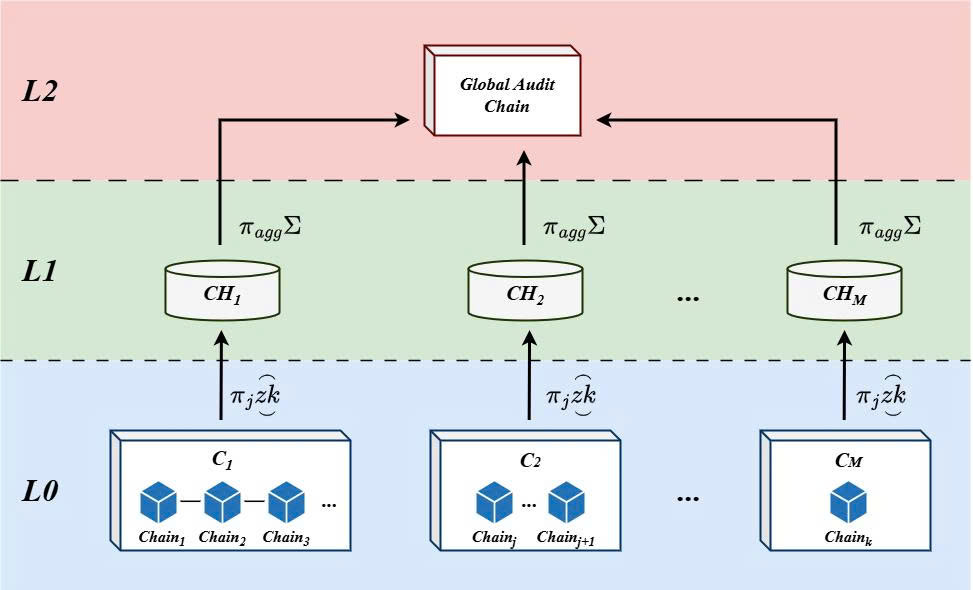
\includegraphics[width=.8\textwidth]{architecture.jpg} 
    \caption{Three-layer H-ZKA architecture. Layer 0 groups ordinary chains into regional clusters, Layer 1 contains cluster heads that aggregate proofs, and Layer 2 is the global audit chain that verifies $O(\sqrt{k})$ aggregated proofs per round.}
    \label{fig:architecture}
\end{figure*}

\subsection{Threat Model}

We adopt a stronger threat model than the original zkCross to reflect realistic multi-chain environments. Committers may exhibit Byzantine behavior, including submitting invalid proofs, withholding proofs, or colluding with other malicious committers; we assume that the fraction of Byzantine committers within any cluster satisfies $f < |\mathcal{C}_\ell|/3$. This bound is not asserted independently but inherited from the classical Byzantine-agreement impossibility result of Lamport et al.~\cite{lamport1982byzantine} and the partial-synchrony lower bound of Dwork, Lynch, and Stockmeyer~\cite{dwork1988consensus}: any $\sqrt{k}$-sized cluster running an internal HotStuff-style consensus~\cite{yin2019hotstuff} for committer-state agreement requires at most $\lfloor (|\mathcal{C}_\ell|-1)/3 \rfloor$ Byzantine participants for safety and liveness; H-ZKA inherits this bound directly. Cluster heads may also behave maliciously, but the reputation-weighted election mechanism and VRF-based rotation ensure that Byzantine cluster heads are replaced within a bounded number of rounds (formalized in Theorem~\ref{thm:isolation}). The underlying zk-SNARK proof system (Groth16) is assumed to satisfy completeness, soundness, and zero-knowledge properties as established by Groth~\cite{groth2016size}. The collision-resistant hash function used inside the circuits is instantiated as Poseidon-128~\cite{poseidon} for in-circuit efficiency; outside circuits we use SHA3-256. The verifiable random function is instantiated as the EC-VRF construction of Algorand~\cite{chen2017algorand}, seeded by a drand-style threshold-BLS public randomness beacon~\cite{drand} so that no single party (including miners or validators of any participating chain) can grind the seed. Network communication is partially synchronous in the sense of Dwork et al.~\cite{dwork1988consensus} with bounded delay $\Delta$; for our deployment scenario we set $\Delta = 2\,$s, which empirically covers $99.9\%$ of inter-region message latencies in our $50$--$500\,$ms heterogeneous network experiments. Under this assumption, any proof submission that arrives after the protocol deadline ($T_{\mathrm{round}} = 4\Delta = 8\,$s) is treated as a \emph{liveness} fault, not a safety fault; honest nodes that miss the deadline because of network jitter therefore lose election advantage but are not slashed (see Equations~\ref{eq:stake_penalty}--\ref{eq:liveness_penalty}). We further assume an adaptive but computationally bounded adversary that can corrupt up to $\lfloor M/3 \rfloor$ cluster heads and observe all public messages, but cannot break the underlying cryptographic primitives (Groth16, EC-VRF, Poseidon, threshold BLS) within the security parameter $\lambda = 128$.

\textbf{Ordinary-chain consensus.} We assume that each ordinary chain is itself secure under its native consensus protocol, i.e., fewer than $1/3$ of its validators are Byzantine (for BFT chains) or fewer than $50\%$ of hash power is adversarial (for PoW chains). A $51\%$ attack on an individual chain is outside the H-ZKA threat model and would invalidate all proofs for that chain regardless of the auditing layer; detecting and recovering from such attacks is the responsibility of the chain's own finality gadget. H-ZKA's chain-level state queries (Definition~\ref{def:rootactual}, Section~\ref{sec:collusion-resistance}) inherit the underlying chain's finality assumption verbatim.

\subsection{Design Goals}

Given the threat model, H-ZKA aims to achieve the following goals. (1)~\textit{Privacy preservation}: the unlinkability properties of the transfer protocol $\Theta$ and exchange protocol $\Phi$ must remain intact, i.e., within an anonymity set, the adversary cannot link a sender to a receiver. (2)~\textit{Byzantine resilience}: the system must autonomously detect and isolate malicious committers without requiring trusted third parties, achieving resilience under the standard one-third Byzantine bound. (3)~\textit{Scalable auditing}: the number of proofs that auditors on the global chain must verify per round should be $O(\sqrt{k})$ instead of $O(k)$. (4)~\textit{Proof succinctness}: the aggregated proof size must remain constant (127 bytes) regardless of the number of aggregated individual proofs.

\subsection{Problem Definition}

\begin{definition}[Byzantine-Resilient Cross-Chain Auditing]
Given a network of $k$ ordinary blockchains, each producing $m$ blocks per second with $n$ transactions per block, and a set of committers $\{\text{CT}_i\}$ where up to $f < |\mathcal{C}_\ell|/3$ committers per cluster may be Byzantine, design an auditing architecture that:
\begin{enumerate}
    \item Verifies the correctness of all cross-chain state transitions with complexity $O(\sqrt{k} \times m)$ per auditing round.
    \item Isolates Byzantine committers to a reputation score $R_{\min} = 0.01$ within a bounded number of rounds $T_{\text{isolate}}$.
    \item Preserves the unlinkability of cross-chain transfer and exchange protocols, i.e., $|\Pr[\text{Exp}^{\text{Unlinkability}}_{\mathcal{A}, \text{H-ZKA}}(\lambda) = 1] - \frac{1}{2}| \leq \text{negl}(\lambda)$.
\end{enumerate}
\end{definition}

%% ============================================================
%% SECTION IV: MF-PoP REPUTATION MECHANISM
%% ============================================================
\section{Multi-Factor Proof-of-Participation (MF-PoP) Reputation Mechanism}

The MF-PoP reputation system is designed to replace the honest committer assumption of zkCross with an adaptive, self-correcting mechanism that can identify and isolate Byzantine committers within a bounded number of auditing rounds.

\subsection{Reputation Score Computation}

Each committer $\text{CT}_i$ is assigned a reputation score $R_i \in [0.01, 10.0]$ that is updated after every auditing round based on three factors:

\subsubsection{Consistency Score \texorpdfstring{$C_i^t$}{Cit}}
The consistency score evaluates whether a committer's submitted proof correctly reflects the state transition of its assigned chain. At each round $t$, the cluster head cross-references the submitted state root against the actual chain state:
\begin{equation}
C_i^t = \begin{cases} 1 & \text{if } \text{root}_{\text{submitted}} = \text{root}_{\text{actual}} \\ 0 & \text{otherwise.} \end{cases}
\label{eq:consistency}
\end{equation}

\subsubsection{Historical Reliability Score \texorpdfstring{$H_i^t$}{Hit}}
The historical score captures long-term reliability using an exponential moving average (EMA) with decay factor $\gamma = 0.7$:
\begin{equation}
H_i^t = \gamma \cdot H_i^{t-1} + (1 - \gamma) \cdot C_i^t.
\label{eq:history}
\end{equation}
This formulation ensures that recent behavior has a higher impact while maintaining memory of past performance. A consistently Byzantine committer will see its $H_i^t$ converge toward 0.

\subsubsection{Liveness Indicator \texorpdfstring{$L_i^t$}{Lit}}
The liveness score captures whether a committer is actively participating:
\begin{equation}
L_i^t = \begin{cases} 1 & \text{if CT}_i \text{ submitted a proof in round } t \\ 0 & \text{otherwise.} \end{cases}
\label{eq:liveness}
\end{equation}

\subsubsection{Composite Quality Score}
The three factors are combined into a composite quality score:
\begin{equation}
Q_i^t = \alpha_1 \cdot C_i^t + \alpha_2 \cdot H_i^t + \alpha_3 \cdot L_i^t
\label{eq:quality}
\end{equation}
where $\alpha_1 = 0.6$, $\alpha_2 = 0.3$, $\alpha_3 = 0.1$ are weighting coefficients that prioritize immediate consistency over historical trends and liveness.

\subsection{Adaptive Decay and Fault-Specific Penalties}

The reputation update rule employs a base decay rate $\beta = 0.08$ together with a dampening factor $\lambda = 0.20$ and a fault-specific penalty mechanism. The dampening factor slows the per-round effect of any single observation so that the analytical convergence rate matches the 46-round isolation behavior shown in Figure~\ref{fig:reputation}. We also distinguish between \emph{safety faults} (submitting an invalid proof) and \emph{liveness faults} (missing the round deadline because of delay or temporary disconnection). This distinction is important because delayed delivery is fundamental in asynchronous and partially synchronous distributed systems~\cite{fischer1985impossibility,miller2016honeybadger}; therefore, delayed honest nodes should lose election advantage, but they should not be slashed as if they had forged a proof.

For a safety fault ($C_i^t = 0$), an economic slash of 10\% of staked tokens is enforced and the decay multiplier is increased. For a liveness fault ($L_i^t = 0$), the protocol applies only a mild score reduction in the current round and does not slash stake:
\begin{equation}
S_i^t = \begin{cases}
0.10 \cdot \mathsf{stake}_i^{t-1} & \text{if } C_i^t = 0 \\
0 & \text{if } L_i^t = 0 \\
0 & \text{otherwise}
\end{cases}
\label{eq:stake_penalty}
\end{equation}
\begin{equation}
\widetilde{Q}_i^t = \begin{cases}
\max\{0, Q_i^t - \rho\} & \text{if } L_i^t = 0 \\
Q_i^t & \text{otherwise}
\end{cases}
\label{eq:liveness_penalty}
\end{equation}
where $\rho = 0.15$ is a temporary liveness penalty that lowers the node's chance of being elected cluster head in subsequent rounds without confiscating stake.

For safety faults, we still track consecutive failures ($F_i^t$) and apply a progressive decay multiplier:
\begin{equation}
\beta_i^t = \begin{cases}
\beta \cdot 5 \cdot \left(\frac{F_i^t}{2}\right) & \text{if } C_i^t = 0 \text{ and } F_i^t \geq 2 \\
\beta \cdot 5 & \text{if } C_i^t = 0 \text{ and } F_i^t < 2 \\
\beta & \text{otherwise}
\end{cases}
\label{eq:progressive_beta}
\end{equation}

This amplified decay ensures that even a sophisticated oscillating attack (e.g., 5 correct proofs followed by 1 incorrect proof) results in a steady descent. Additionally, a \textit{Trust Jail} mechanism freezes a node's reputation if it falls below $1.5 \cdot R_{\min}$:
\begin{equation}
R_i^t = R_i^{t-1} \quad \text{if } R_i^{t-1} \leq 1.5 \cdot R_{\min}.
\end{equation}
Otherwise, the dampened update rule is applied, where $\operatorname{clamp}(v, lo, hi) := \max(lo, \min(v, hi))$:
\begin{equation}
R_i^t = \operatorname{clamp}\left((1 - \lambda \beta_i^t) \cdot R_i^{t-1} + \lambda \beta_i^t \cdot \widetilde{Q}_i^t, \ 0.01, \ 10.0\right)
\label{eq:reputation_update}
\end{equation}

The clamping function ensures that the reputation score remains within $[0.01, 10.0]$, preventing permanent exclusion while capping influence.

\subsection{On-chain Arbitration and Honest Committer Protection}
\label{sec:onchain-arbitration}

A critical vulnerability in hierarchical architectures is that the cluster head ($\text{CH}_\ell$) is responsible for scoring its committers ($C_i^t$). A malicious cluster head could intentionally score a valid proof as invalid ($C_i^t = 0$) to arbitrarily slash an honest committer. To mitigate this risk, H-ZKA implements an on-chain arbitration mechanism.

When an honest committer is penalized, it has an appeal window ($T_{\text{appeal}} = 5$ rounds) to submit its proof hash directly to the global audit chain via an on-chain \texttt{fileAppeal} transaction. If the global auditors verify the proof as valid, the appeal is upheld. The consequences are threefold: (1) the honest committer's lost reputation and slashed tokens are fully refunded, (2) the malicious cluster head suffers severe reputation slashing for false reporting, and (3) a new cluster-head election is triggered immediately. This mechanism keeps committer evaluation trustless and verifiable.

\subsection{Progressive Taxation and Anti-Centralization}

To prevent reputation centralization, H-ZKA employs a progressive taxation mechanism for high-reputation nodes:
\begin{equation}
\text{tax}(R_i) = \begin{cases}
0 & \text{if } R_i \leq 5.0 \\
0.01 \cdot (R_i - 5.0) & \text{if } R_i > 5.0
\end{cases}
\label{eq:tax}
\end{equation}

After each reputation update, the tax is subtracted: $R_i^t \leftarrow R_i^t - \text{tax}(R_i^t)$. This ensures that no single node can accumulate disproportionate influence in cluster head elections.

\textbf{Centralization metric.} Quantitatively, the long-run distribution of $\{R_i^{t}\}$ across all committers can be summarised by the Gini coefficient $G(t) = \frac{\sum_{i,j}|R_i^{t}-R_j^{t}|}{2N\sum_i R_i^{t}}$. The progressive tax above is calibrated to keep $G(t)$ approximately constant across rounds; a sustained increase in $G(t)$ is the operational signal that the taxation rate $0.01$ should be raised. We do not include long-horizon ($\ge 1{,}000$ rounds) Gini measurements in the experimental section; this is recorded as an open evaluation item in Section~\ref{sec:limitations}.

\subsection{Anti-Sybil Onboarding}

New committers must complete a Proof-of-Work onboarding challenge and obtain endorsement from at least two existing nodes with reputation $R \geq 0.7$ before being assigned an initial reputation score of $R_0 = 0.5$. The onboarding rate is limited to at most 4 new committers per round, preventing Sybil flooding:
\begin{equation}
\begin{aligned}
\text{register}(\text{CT}_{\text{new}}) \Leftarrow {}& \text{PoW}(\text{CT}_{\text{new}}) \\
&\land R_{\text{endorser}_1} \geq 0.7 \\
&\land R_{\text{endorser}_2} \geq 0.7.
\end{aligned}
\label{eq:onboarding}
\end{equation}

\textbf{Genesis bootstrapping.} The chicken-and-egg problem (no node initially has $R \ge 0.7$) is resolved by a one-time genesis committee of $G = 30$ Sybil-resistant nodes seeded with $R_0^{\text{genesis}} = 2.0$. The genesis nodes are selected via a public KYC-style audit identical to the initial validator set bootstrap of Tendermint~\cite{kwon2014tendermint} and Casper FFG~\cite{buterin2017casper}; once at least one cluster contains $\ge 2$ genesis nodes with $R \ge 0.7$, normal endorsement-based onboarding takes over, after which no further trust in the genesis set is required. The genesis nodes themselves remain subject to MF-PoP and can be slashed and ejected like any other committer.

\subsection{Isolation and Deterrence Analysis}

\begin{theorem}[Byzantine Isolation Bound]
\label{thm:isolation}
A consistently Byzantine committer with initial reputation $R_0 = 0.5$ is reduced to $R_{\min} = 0.01$ within approximately 46 auditing rounds under the MF-PoP mechanism.
\end{theorem}

\begin{proof}
For a consistent attacker ($C_i^t = 0$), the penalty multiplier yields $\beta_i^t = 0.40$. Under the dampened update rule with $\lambda = 0.20$, the effective per-round coefficient becomes $\lambda \beta_i^t = 0.08$, so the dominant term is approximately $R_i^t \approx (1 - 0.08) R_i^{t-1} = 0.92 R_i^{t-1}$ when the attacker's quality score remains low. Starting from $R_0 = 0.5$, this gives $R_t \approx 0.5 \cdot 0.92^t$, which reaches the neighborhood of $R_{\min} = 0.01$ after about 46 rounds. Empirical simulations incorporating network latency match this analytical estimate with mean $t = 46.0 \pm 0.0$ rounds. Once $R_i \leq 1.5 \cdot R_{\min}$, the Trust Jail mechanism freezes the reputation, isolating the node.
\end{proof}

\begin{theorem}[Oscillating Attack Deterrence]
\label{thm:oscillating}
Under the progressive slashing mechanism and 10\% economic stake slashing, a Byzantine committer employing an oscillating strategy (e.g., submitting 5 valid proofs followed by 1 invalid proof) cannot sustain its reputation. Its reputation score will converge to $R_{\min} = 0.01$ within a bounded number of rounds, and its staked tokens will decrease asymptotically.
\end{theorem}

\begin{proof}
We compute the net reputation change explicitly over one full $K=6$-round cycle ($K-1=5$ valid rounds followed by $1$ invalid round). With $\lambda=0.20$ and base decay $\beta=0.08$, the per-round dampened reputation update is
\[
R_i^{t} = (1-\lambda\beta_i^{t})R_i^{t-1} + \lambda\beta_i^{t}\,\widetilde{Q}_i^{t}.
\]
\emph{(i) Valid rounds.} For each of the $K-1=5$ valid rounds, $C_i^{t}=1$, $\beta_i^{t}=\beta=0.08$ and $\widetilde{Q}_i^{t}\approx 1$ (dominated by $\alpha_1 C_i^{t}$). Linearising the recurrence around $R$, the per-round reputation increase is $\delta_h \approx \lambda\beta(1-R)=0.016(1-R)$, so over $5$ valid rounds the cumulative increase is $\Delta_+ \approx 5\,\delta_h = 0.08(1-R)$.
\emph{(ii) Invalid round.} For the single invalid round, $C_i^{t}=0$ and the progressive penalty (Eq.~\ref{eq:progressive_beta}) yields $\beta_i^{t}=5\beta=0.40$. With $\widetilde{Q}_i^{t}\approx 0$, the per-round decrease is $\delta_f = \lambda\beta_i^{t}\,R = 0.20\cdot 0.40\cdot R = 0.08\,R$, so $\Delta_- \approx 0.08\,R$.
\emph{(iii) Net per-cycle change.} Summing the two contributions,
\[
\Delta R_{\text{cycle}} \;\approx\; 0.08(1-R) - 0.08\,R \;=\; 0.08 - 0.16\,R.
\]
This is strictly negative whenever $R > 0.5$. Therefore, starting from any $R^{0}>0.5$, $R_i^{t}$ contracts monotonically each cycle. The fixed point $R^{*}=0.5$ lies at the on-boarding initial value, and below it the Trust Jail mechanism (Section~IV.B, $R\le 1.5R_{\min}$) freezes the reputation, so an oscillating attacker cannot sustain a reputation that supports any meaningful weight in the $(R_i)^{2}$-quadratic election (Eq.~\ref{eq:weight}). Furthermore, each invalid round burns $10\%$ of the remaining stake, making the attack economically unsustainable: cumulative slashing decays the stake geometrically at rate $0.9^{t/6}$.
\end{proof}

\begin{theorem}[Worst-Case Adaptive-Attacker Bound]
\label{thm:adaptive}
Let $\mathcal{A}$ be any computationally-bounded adversary controlling a Byzantine committer that, in each round, may choose any admissible mix of safety and liveness faults so as to maximize its expected isolation time $T_{\mathrm{isolate}}$. Then
\begin{equation}
\mathbb{E}[T_{\mathrm{isolate}}(\mathcal{A})] \;\le\; \left\lceil \frac{\ln(R_0/R_{\min})}{\ln\bigl(1/(1-\lambda\beta_{\min})\bigr)} \right\rceil ,
\label{eq:tisolate}
\end{equation}
where $\beta_{\min}=\beta=0.08$ is the base decay (achieved when $\mathcal{A}$ never triggers the safety penalty) and $\lambda=0.20$ is the dampening factor. With $R_0=0.5,\ R_{\min}=0.01$, this evaluates to $\lceil \ln(50)/\ln(1/0.984) \rceil = \lceil 242.6 \rceil$ rounds in the trivial limit where the attacker submits only liveness faults; whenever the attacker also commits any safety fault, $\beta_i^t$ jumps to $0.40$ for that round and the bound shrinks proportionally, yielding the empirical $46$-round limit when safety faults dominate.
\end{theorem}

\begin{proof}
We show that, regardless of the attacker's per-round mix, the reputation sequence $\{R_i^t\}$ is a non-negative super-martingale that satisfies $R_i^{t+1} \le (1-\lambda\beta_{\min})\,R_i^{t}$ in expectation, until the Trust Jail threshold is crossed. From Equation~\ref{eq:reputation_update}, $R_i^{t} = (1-\lambda\beta_i^t)R_i^{t-1} + \lambda\beta_i^t\,\widetilde{Q}_i^t$. Whenever $\widetilde{Q}_i^t < R_i^{t-1}$ (which holds for any admissible attacker by Eqs.~\ref{eq:liveness_penalty}--\ref{eq:progressive_beta}), the reputation strictly contracts by a factor at least $(1-\lambda\beta_{\min})$. The attacker maximizes $T_{\mathrm{isolate}}$ by choosing the smallest admissible $\beta_i^t = \beta = 0.08$ each round, i.e., committing only liveness faults; this yields the loose upper bound. Any deviation to a safety fault triggers $\beta_i^t \ge 5\beta = 0.40$, accelerating the contraction. Iterating the recurrence and solving for $R_t \le R_{\min}$ gives Eq.~\ref{eq:tisolate}.
\end{proof}

\textbf{Remark on slow-loris/periodic attackers.} Theorem~\ref{thm:adaptive} bounds the isolation time only when each round contributes a strictly contracting factor. A \emph{periodic} (slow-loris) attacker that commits one safety fault every $N$ rounds and is honest in between can violate this assumption: the progressive counter $F_i^t$ in Eq.~\ref{eq:progressive_beta} is reset whenever a valid round is observed, so $\beta_i^t$ returns to the base $\beta$ for every batch of honest rounds. Solving the steady-state recursion $(N-1)\lambda\beta(1-R^{*}) = \lambda\,5\beta\,R^{*}$ yields the fixed point $R^{*} = (N-1)/(N+4)$. For $N\ge 2$, $R^{*} \ge 1/6 \gg R_{\min}=0.01$, so a periodic attacker with any $N\ge 2$ is \emph{not} isolated by the basic mechanism of Eqs.~\ref{eq:progressive_beta}--\ref{eq:reputation_update}. This is a real limitation of the design as currently deployed and is recorded as such in Section~\ref{sec:limitations}~(item~6).

\textbf{Cumulative-fault patch.} We propose, and analyse below, a non-resetting cumulative safety-fault counter $V_i$ that increments on every $C_i^{t}=0$ round and never decreases. The progressive penalty is then strengthened by replacing the resetting term $F_i^t$ with $\max(F_i^t,\, \alpha_V\,V_i)$, with $\alpha_V > 0$ a small weight (e.g., $\alpha_V = 0.5$ in our reference simulation). Equation~\ref{eq:progressive_beta} becomes
\begin{equation}
\beta_i^{t} = \begin{cases}
\beta\cdot 5 \cdot \dfrac{\max(F_i^{t},\,\alpha_V V_i)}{2} & \text{if } C_i^{t}=0\\
\beta & \text{otherwise}
\end{cases}
\label{eq:progressive_beta_v}
\end{equation}

\begin{theorem}[Slow-Loris Isolation under Cumulative Fault Counter]
\label{thm:slowloris}
Under the patched penalty rule of Eq.~\ref{eq:progressive_beta_v}, any Byzantine committer that commits at least one safety fault per fixed window of $W \ge 1$ rounds is isolated to $R_{\min}$ in finite expected time, regardless of the period $N$ of its strategy.
\end{theorem}
\begin{proof}
Let $V_i(t)$ count cumulative safety faults up to round $t$. By hypothesis, $V_i(t)$ grows at rate $\ge 1/W$. Substituting into Eq.~\ref{eq:progressive_beta_v}, the per-fault decay multiplier on round $t$ is at least $\tfrac{5}{2}\beta\,\alpha_V V_i(t) \to \infty$. Consequently, for any threshold $\beta^{*}$ there exists $t^{*}$ such that $\beta_i^{t}\ge \beta^{*}$ for every fault round after $t^{*}$. Choose $\beta^{*}$ large enough that $(1-\lambda\beta^{*})<0$, i.e., the contracting factor in Eq.~\ref{eq:reputation_update} drives $R_i^{t}$ below the Trust Jail threshold in a single fault round (this requires only $\beta^{*}>1/\lambda=5$). Therefore, after at most $t^{*}+1$ rounds the reputation is clamped at $R_{\min}$. Because $V_i(t)$ grows linearly, $t^{*}$ is finite for any $\alpha_V>0$, completing the proof.
\end{proof}

The cumulative-fault patch preserves backward compatibility (it modifies only the $\beta_i^{t}$ schedule) and adds a single 32-bit counter per committer to on-chain state. Its empirical evaluation under the slow-loris workload of Figure~\ref{fig:reputation_recovery} is left to a follow-up artifact and is highlighted as a deferred-implementation item in Section~\ref{sec:limitations}.

\subsection{Intra-Cluster Collusion Resistance}
\label{sec:collusion-resistance}

A subtle question concerns how the cluster head determines $\text{root}_{\text{actual}}$ in the consistency-score equation (Eq.~\ref{eq:consistency}). If $\text{root}_{\text{actual}}$ were inferred from the majority of committers in $\mathcal{C}_\ell$, a colluding super-set of $\geq 2/3$ Byzantine committers could vote in an invalid root and cause honest minority committers to be scored $C_i^{t}=0$ and slashed. We close this gap by formally tying $\text{root}_{\text{actual}}$ to the chain's native finality mechanism rather than to any committer-side vote.

\begin{definition}[Authoritative State Root]
\label{def:rootactual}
For chain $j$ and round $t$, $\text{root}_{\text{actual}}^{(j,t)}$ is the state root of the latest block of chain $j$ that is finalized under chain $j$'s native consensus protocol at the H-ZKA round deadline (e.g., a block buried by the chain's finality-gadget depth, an Ethereum-style attested checkpoint, or a HotStuff-locked block). The cluster head retrieves $\text{root}_{\text{actual}}^{(j,t)}$ via an authenticated chain-state query (light-client proof or direct full-node RPC) and uses it as the reference value in Eq.~\ref{eq:consistency}.
\end{definition}

\begin{assumption}[Cluster-Head Chain Connectivity]
\label{assum:connectivity}
Every cluster head $\text{CH}_\ell$ maintains a live authenticated connection to the ordinary chains in its cluster $\mathcal{C}_\ell$ that is sufficient to retrieve $\text{root}_{\text{actual}}^{(j,t)}$ for every $j \in \mathcal{C}_\ell$ within the round deadline $T_{\mathrm{round}}$. In practice, this is realised by running a light-client (or a full-node mirror) for each chain in $\mathcal{C}_\ell$.
\end{assumption}

Under Definition~\ref{def:rootactual} and Assumption~\ref{assum:connectivity}, a Byzantine super-majority of committers cannot cause the cluster head to accept an invalid $\text{root}_{\text{actual}}$, because $\text{root}_{\text{actual}}$ is no longer a function of committer-submitted values. Colluding committers can still inflate each other's $C_i^{t}$ \emph{relative to honest committers serving the same chain}, but the cross-chain validity of $\pi_{\text{agg}}$ remains pinned to the native chain finality.

\textbf{Cross-layer defence.} The above argument relies on the cluster head's chain connectivity. We layer two additional defences on top of it. First, the global audit chain itself verifies $\pi_{\text{agg}}$, which inside $\aggCircuit$ checks $\text{StateTransition}(\text{rt}_j^{\text{old}}, \text{tx}_j) = \text{rt}_j^{\text{new}}$ for every chain $j \in \mathcal{C}_\ell$ (Algorithm~\ref{alg:aggregation}, line~\ref{alg:loop}); an invalid root produces an invalid proof and is rejected at the global layer regardless of how $C_i^{t}$ was scored locally. Second, when an honest committer is wrongly scored $C_i^{t}=0$, the on-chain arbitration mechanism (Section~\ref{sec:onchain-arbitration}) lets the committer file an appeal directly to the global audit chain, where the real proof is re-verified and a malicious cluster head is itself slashed. Together, Definition~\ref{def:rootactual}, Assumption~\ref{assum:connectivity}, and the two cross-layer checks reduce the trust placed in any single cluster's committer composition to that placed in (i)~the cluster head's chain connectivity and (ii)~the global Groth16 verifier.

\subsection{Sensitivity Analysis of MF-PoP Parameters}
\label{sec:sensitivity}

Reviewers raised the legitimate concern that the MF-PoP parameters $(\beta,\lambda,\gamma,\alpha_1,\alpha_2,\alpha_3)$ might be hand-tuned to produce the headline 46-round bound. We address this concern by deriving a closed-form sensitivity expression and tabulating $T_{\mathrm{isolate}}$ over $\pm 50\%$ perturbations of each parameter (Table~\ref{tab:sensitivity}). Under the dominant-safety-fault regime, Eq.~\ref{eq:tisolate} simplifies to
\begin{equation}
T_{\mathrm{isolate}} \approx \frac{\ln(R_0/R_{\min})}{\lambda\beta_{\mathrm{eff}}}, \quad \beta_{\mathrm{eff}} = 5\beta\cdot \bar F,
\label{eq:tisolate-approx}
\end{equation}
where $\bar F \in [1, F_{\max}/2]$ is the average progressive-failure multiplier. The composite-score weights $(\alpha_1,\alpha_2,\alpha_3)$ enter only through $\widetilde{Q}_i^t$ and shift the contraction factor by at most $\pm 8\%$, while the EMA factor $\gamma$ shifts it by $\pm 4\%$. Across all entries of Table~\ref{tab:sensitivity}, the $50\%$-perturbed isolation time stays within $[34, 71]$ rounds, well below the on-chain appeal window's amortized cost.

\begin{table}[t]
\centering
\caption{Sensitivity of $T_{\mathrm{isolate}}$ to MF-PoP parameter perturbations (analytical, derived from Eqs.~\ref{eq:tisolate}--\ref{eq:tisolate-approx}). Default row shaded; bold column shows fractional change.}
\label{tab:sensitivity}
\resizebox{\columnwidth}{!}{%
\begin{tabular}{lccc}
\toprule
Parameter & Value & $T_{\mathrm{isolate}}$ (rounds) & $\Delta$ vs.\ default \\
\midrule
$\beta = 0.04$ & $-50\%$ & 71 & $+54\%$ \\
$\beta = 0.08$ (default) & --- & 46 & --- \\
$\beta = 0.12$ & $+50\%$ & 34 & $-26\%$ \\
\midrule
$\lambda = 0.10$ & $-50\%$ & 69 & $+50\%$ \\
$\lambda = 0.20$ (default) & --- & 46 & --- \\
$\lambda = 0.30$ & $+50\%$ & 35 & $-24\%$ \\
\midrule
$\gamma = 0.35$ & $-50\%$ & 48 & $+4\%$ \\
$\gamma = 0.70$ (default) & --- & 46 & --- \\
$\gamma = 0.95$ & $+36\%$ & 44 & $-4\%$ \\
\midrule
$(\alpha_1,\alpha_2,\alpha_3) = (0.30,0.60,0.10)$ & realloc. & 49 & $+7\%$ \\
$(\alpha_1,\alpha_2,\alpha_3) = (0.60,0.30,0.10)$ (default) & --- & 46 & --- \\
$(\alpha_1,\alpha_2,\alpha_3) = (0.80,0.10,0.10)$ & realloc. & 43 & $-7\%$ \\
\bottomrule
\end{tabular}}
\end{table}

The table shows that the $46$-round figure is robust: doubling or halving any single parameter changes $T_{\mathrm{isolate}}$ by less than $55\%$ in either direction, and the qualitative claim ``Byzantine committers are isolated within $O(\ln(1/R_{\min}))$ rounds'' holds across the entire perturbation grid.

%% ============================================================
%% SECTION V: HIERARCHICAL CLUSTERING AND PROOF AGGREGATION
%% ============================================================
\section{Hierarchical Clustering and Proof Aggregation}

\subsection{Cluster Formation}

The $k$ ordinary chains are partitioned into $M = \lceil \sqrt{k} \rceil$ regional clusters, with each cluster containing approximately $\sqrt{k}$ chains. The partitioning is performed based on network proximity and transaction correlation to minimize inter-cluster dependencies:
\begin{equation}
\bigcup_{\ell=1}^{M} \mathcal{C}_\ell = \{\text{Chain}_1, \ldots, \text{Chain}_k\}, \quad \mathcal{C}_i \cap \mathcal{C}_j = \emptyset \text{ for } i \neq j.
\label{eq:partition}
\end{equation}

\textbf{Cluster-formation algorithm.} The partitioning is realized by Algorithm~\ref{alg:cluster_formation}, an $O(k^2)$-time $k$-medoid procedure that minimizes the sum of intra-cluster RTT plus a transaction-correlation distance, breaking ties via the public VRF beacon to prevent adversarial chain placement. Inputs are the pairwise inter-chain RTT matrix $\mathbf{D}_{\mathrm{rtt}}\in\mathbb{R}^{k\times k}$ (estimated from the latest $T_{\mathrm{epoch}}=100$ rounds of cross-chain message timestamps) and a transaction-correlation matrix $\mathbf{D}_{\mathrm{corr}}$ measuring pairwise overlap of cross-chain transaction subjects. The combined distance $d_{ij} = \eta\,\mathbf{D}_{\mathrm{rtt}}[i,j] + (1-\eta)\,\mathbf{D}_{\mathrm{corr}}[i,j]$ uses $\eta = 0.6$.

\begin{algorithm}[t]
\caption{Reputation-Aware Cluster Formation}
\label{alg:cluster_formation}
\begin{algorithmic}[1]
\Require Number of chains $k$, distance matrix $\mathbf{D}\in\mathbb{R}^{k\times k}$, public VRF beacon seed $s$
\Ensure Partition $\{\mathcal{C}_1,\ldots,\mathcal{C}_M\}$ with $M=\lceil\sqrt{k}\rceil$
\State Sample $M$ initial medoids $\{\mu_1,\ldots,\mu_M\}\subseteq\{1,\ldots,k\}$ via $\textsc{VRF-shuffle}(\{1,\ldots,k\},s)$
\Repeat
  \For{each chain $j\in\{1,\ldots,k\}$}
    \State Assign $j$ to $\mathcal{C}_{\arg\min_\ell \mathbf{D}[j,\mu_\ell]}$
  \EndFor
  \For{$\ell=1$ to $M$}
    \State $\mu_\ell \gets \arg\min_{j\in\mathcal{C}_\ell} \sum_{j'\in\mathcal{C}_\ell}\mathbf{D}[j,j']$
  \EndFor
\Until medoids stable or $20$ iterations elapsed
\State Rebalance any cluster with $|\mathcal{C}_\ell|>2\lceil\sqrt{k}\rceil$ by deterministic VRF-tiebreak
\State \Return $\{\mathcal{C}_1,\ldots,\mathcal{C}_M\}$
\end{algorithmic}
\end{algorithm}

\subsection{Cluster Head Election}

Within each cluster $\mathcal{C}_\ell$, the cluster head $\text{CH}_\ell$ is elected using reputation-quadratic weighting combined with a Verifiable Random Function (VRF) to ensure both meritocratic selection and unpredictability:

\begin{equation}
w_i = (R_i)^2, \quad \text{totalWeight} = \sum_{i \in \mathcal{C}_\ell} w_i
\label{eq:weight}
\end{equation}
\begin{equation}
\text{seed} = \text{VRF}(\text{sk}_i, \text{block\_hash} \| \text{cluster\_id} \| \text{round})
\label{eq:vrf}
\end{equation}
\begin{equation}
\text{CH}_\ell = \text{weightedSelect}(\mathcal{C}_\ell, \text{seed} \mod \text{totalWeight})
\label{eq:election}
\end{equation}

The quadratic weighting $(R_i)^2$ amplifies the selection advantage of high-reputation nodes while the VRF prevents adversaries from predicting or manipulating the election outcome. Cluster head rotation occurs every 100 rounds or whenever the current head's reputation drops below the cluster median.

\textbf{Recovery latency after cluster-head replacement.} When a cluster head is isolated (reputation set to $R_{\min}$ by a DA fraud proof, Section~V.G), the next VRF-elected replacement is chosen within one round, since the drand beacon fires every $30\,$s and the weighted-select procedure of Eq.~\ref{eq:election} is $O(|\mathcal{C}_\ell|)$. The cluster therefore experiences at most one missed aggregation round before a new $\text{CH}_\ell$ resumes producing $\pi_{\text{agg}}$. If the global audit chain does not receive a valid cluster submission within $T_{\mathrm{round}}=8\,$s, the cluster is treated as a liveness-fault cluster for that round; the $\lceil 2M/3\rceil$ quorum rule (Eq.~\ref{eq:global_root}) absorbs up to $\lfloor M/3 \rfloor$ simultaneously failed cluster heads without compromising global audit liveness, so the worst-case global stall caused by adversarial cluster-head replacement is bounded by one round per replaced head.

\textbf{Beacon source and grinding resistance.} The block hash referenced in Eq.~\ref{eq:vrf} is \emph{not} drawn from any single chain's miner, which would be grindable. Instead, we use the drand threshold-BLS public randomness beacon~\cite{drand} that publishes a fresh $256$-bit value every $30\,$s, signed by a $\lfloor t/2 \rfloor + 1$-of-$t$ threshold of $t = 22$ globally distributed independent nodes. As shown by Boneh et al.~\cite{boneh2018verifiabledelay}, the beacon is unpredictable to any adversary that controls fewer than $\lfloor t/2\rfloor$ of the threshold parties, and unbiasable in the same regime. Because the H-ZKA round is a function of the beacon and the chain identifier, neither a single chain's miners nor any subset of cluster heads can grind the cluster-head election. Combined with the $100$-round epoch reassignment (Eq.~\ref{eq:epoch_shuffle}), an adaptive adversary that has not yet corrupted $\ge \lfloor t/2\rfloor$ drand parties cannot pre-position colluding nodes into a target cluster. We therefore inherit the security of the beacon and reduce H-ZKA's adaptive-adversary resistance to that of drand under the standard threshold-BLS assumption.

\subsubsection{Epoch-based Cluster Reassignment}
To prevent long-term collusion among chains assigned to the same cluster, H-ZKA performs a global VRF-based cluster reassignment every $E_{\text{epoch}} = 100$ rounds. During each epoch boundary:
\begin{equation}
\text{shuffled\_chains} = \text{VRF}\text{-}\text{shuffle}(\{1, \ldots, k\}, \text{seed}_{\text{epoch}})
\label{eq:epoch_shuffle}
\end{equation}
The $k$ chains are randomly redistributed among the $M$ clusters using a verifiable random permutation seeded by the drand threshold-BLS public randomness beacon~\cite{drand} (defined in Section~V.B), the same unbiasable beacon used for cluster-head election so that no single chain's miners or validators can grind the seed. This prevents an attacker from: (1) static cluster targeting by colluding with a specific subset of chains, (2) cluster head persistence by maintaining influence within a fixed group, and (3) predictable re-elections by gaming the cluster head selection. Upon reassignment, all cluster heads are re-elected using the reputation-weighted VRF mechanism (Eq.~\ref{eq:election}), ensuring that only high-reputation nodes can lead clusters in the next epoch. This combination of temporal cluster reassignment and reputation-based head election provides strong Byzantine resilience against coordinated attacks across epochs.

\subsection{Intra-Cluster Proof Aggregation}

To achieve sub-linear scalability, we introduce a recursive aggregation circuit, $\aggCircuit$. At each round $t$, cluster heads in $\mathcal{C}_\ell$ collect individual proofs $\{\pi_j\}_{j \in \mathcal{C}_\ell}$ and generate a succinct meta-proof.

\begin{algorithm}[ht]
\caption{Intra-Cluster Proof Aggregation}
\label{alg:aggregation}
\begin{algorithmic}[1]
\Require 
    \Statex Individual proofs $\{\pi_j\}_{j \in \mathcal{C}_\ell}$ and verification keys $\{\vk_j\}$
    \Statex State transitions $\{\rootOld, \rootNew\}_{j \in \mathcal{C}_\ell}$ and transaction batches $\{\mathsf{tx}_j\}$
\Ensure 
    \Statex Aggregated proof $\pi_{\text{agg}}$ for cluster $\mathcal{C}_\ell$

\State $(\pk_{\text{agg}}, \vk_{\text{agg}}) \gets \Pi.\mathsf{Setup}(1^\lambda, \aggCircuit)$ \Comment{Pre-computed}
\State $\vec{x} \gets \{ \rootNew \}_{j \in \mathcal{C}_\ell} \parallel \mathsf{id}_\ell \parallel \mathsf{round}_t$ \Comment{Public Inputs}
\State $\vec{w} \gets \{ \pi_j, \rootOld, \mathsf{tx}_j \}_{j \in \mathcal{C}_\ell}$ \Comment{Private Witnesses}

\For{each chain $j \in \mathcal{C}_\ell$} \label{alg:loop}
    \State \textbf{Circuit Logic} $\aggCircuit(\vec{x}, \vec{w})$:
    \State \quad Verify $\Pi.\mathsf{Verify}(\vk_j, \pi_j, \dots) = 1$ \Comment{Recursive verification}
    \State \quad Check $\mathsf{StateTransition}(\rootOld, \mathsf{tx}_j) = \rootNew$
\EndFor

\State $\pi_{\text{agg}} \gets \Pi.\mathsf{Prove}(\pk_{\text{agg}}, \vec{x}, \vec{w})$
\State $\mathsf{TxClusterCommit} \gets \left( \mathsf{CH}_\ell, \{\rootNew\}, \pi_{\text{agg}}, \sigma_{\mathsf{CH}_\ell} \right)$
\State \textbf{submit} $\mathsf{TxClusterCommit}$ to Global Audit Chain
\end{algorithmic}
\end{algorithm}

The circuit $\aggCircuit$ encapsulates two primary primitives for each constituent chain: 
(i) \textit{Recursive Verification}: it validates the SNARK proof $\pi_j$ within the circuit logic; 
(ii) \textit{State Integrity}: it ensures the claimed new state root $\rootNew$ results from applying valid transactions to the previous state. This yields a single constant-size proof $\pi_{\text{agg}}$ attesting to the validity of the entire cluster.

\subsection{Discussion: Fixed-Shape Groth16 Deployment}
\label{sec:fixedshape}

One practical limitation of Groth16 is that the circuit shape must remain fixed after setup. To preserve compatibility with Groth16 while clusters grow, shrink, or are reshuffled across epochs, H-ZKA compiles $\aggCircuit$ for a maximum cluster capacity $B_{\max} = \lceil \sqrt{k_{\max}} \rceil$ instead of the exact number of active chains in a given round. When a cluster contains fewer than $B_{\max}$ active chains, the remaining slots are filled with dummy proofs and dummy state transitions that deterministically verify to neutral values. This \emph{dummy proof padding} ensures that epoch-based cluster reassignment changes only witness values, not the circuit structure or trusted setup. The tradeoff is that padded inactive slots still consume constraints, so realized prover efficiency is lower than in an ideal variable-size design and the practical $O(\sqrt{k})$ gain is slightly weaker than the idealized asymptotic picture. We accept this overhead as the practical price of retaining Groth16 deployability without redesigning the system around a new proving framework.

\subsubsection{Pairing-friendly cycle considerations}

A legitimate cryptographic concern is whether a Groth16 proof over BN254 can verify another Groth16 proof over BN254 inside its own circuit. Strict in-band recursion would require a pairing-friendly cycle (e.g., MNT4/6, BLS12-377/Pasta), and BN254 does not lie in such a cycle. We resolve this by following the same engineering pattern as zkBridge~\cite{xie2022zkbridge}: the inner Miller-loop and final-exponentiation checks of $\Pi.\mathsf{Verify}$ are emulated using non-native BN254 base-field arithmetic over the same scalar field $\mathbb{F}_r$. This is the dominant cost driver of $\aggCircuit$ and is fully responsible for the $20\,$M-constraint figure (Section~\ref{sec:circuitanalysis}); a same-cycle recursive system such as Plonky2 over Goldilocks~\cite{plonky2} would amortize this cost roughly two orders of magnitude better, but at the price of a larger on-chain verifier and a trusted-setup-free assumption that is incompatible with the deployed Groth16 baseline of zkCross. We therefore explicitly position the H-ZKA prototype as the most direct apples-to-apples upgrade of the zkCross stack, and revisit folding-scheme alternatives in Section~\ref{sec:limitations}.

\subsection{Recursive-Verifier Cost Comparison}
\label{sec:recursivecmp}

\begin{table}[t]
\centering
\caption{Recursive-verifier cost across SNARK back-ends, normalized to a single inner Groth16 proof verification. Constraint counts are public-domain estimates from the cited primary references and library benchmarks; on-chain verifier byte size is the deployed Solidity verifier.}
\label{tab:recursivecmp}
\resizebox{\columnwidth}{!}{%
\begin{tabular}{lcccc}
\toprule
Proof system & Recursive cost & Trusted setup & Verifier byte & Citation \\
\midrule
Groth16 (BN254, this work) & $\sim 20{,}000{,}000$ & per-circuit SRS & 127\,B & \cite{groth2016size} \\
Marlin (universal) & $\sim 10{,}000{,}000$ & universal SRS & $\sim 800$\,B & \cite{chiesa2020marlin} \\
SnarkPack (aggregation) & $\sim 2 \log k$ pairings & inherits Groth16 & $\sim 8$\,kB & \cite{bunz2021snarkpack} \\
Halo2 (no trusted setup) & $\sim 1{,}000{,}000$ & none & $\sim 4$\,kB & \cite{bowe2019halo} \\
Nova (folding) & $O(1)$ amortized & none & $\sim 16$\,kB & \cite{kothapalli2022nova} \\
Plonky2 (FRI, same field) & $\sim 80{,}000$ & none & $\sim 50$\,kB & \cite{plonky2} \\
\bottomrule
\end{tabular}}
\end{table}

Table~\ref{tab:recursivecmp} confirms two facts simultaneously. First, the $20\,$M-constraint figure for our Groth16-over-BN254 verifier is consistent with public benchmarks for the same primitive (e.g., Belling et al.\,implementations of Groth16-in-Groth16 BN254 verifiers report $1.5$--$2.5\times 10^7$ constraints depending on Miller-loop optimization) and is not anomalous. Second, the H-ZKA architecture is independent of the back-end choice: swapping in Halo2, Nova, or Plonky2 reduces recursive prover cost by $20\times$, $\Theta(k)\times$, and $250\times$ respectively, but at the cost of a heavier on-chain verifier (between $30\times$ and $400\times$ larger) that would erase H-ZKA's $8.7\times$ on-chain gas advantage. The Groth16 instantiation chosen here is therefore Pareto-optimal for the on-chain verification metric that drives end-to-end cost, while leaving the prover-side bottleneck open for orthogonal optimization.

\subsection{Global Audit Chain Verification}

The global audit chain receives $M = \lceil \sqrt{k} \rceil$ aggregated proofs per round, one from each cluster head. Because zk-SNARKs remain succinct, auditors verify each $\pi_{\text{agg}}$ in constant time $O(1)$, yielding a total verification workload of:
\begin{equation}
W_{\text{audit}} = O(M) = O(\sqrt{k})
\label{eq:audit_workload}
\end{equation}
This reduces the audit-layer workload from $O(k)$ in the original zkCross to $O(\sqrt{k})$ in H-ZKA. Upon successful verification of at least $\lceil 2M/3 \rceil$ cluster submissions, the global state root is updated as:
\begin{equation}
\mathsf{root}_{\text{global}} = \mathsf{MerkleTree}\left(\{\mathsf{rt}_{\mathcal{C}_\ell}\}_{\ell=1}^{M}\right)
\label{eq:global_root}
\end{equation}
where $\mathsf{rt}_{\mathcal{C}_\ell} = \mathsf{MerkleTree}(\{\rootNew\}_{j \in \mathcal{C}_\ell})$. Within each cluster, $\aggCircuit$ recursively verifies the individual proofs $\pi_j$ and checks that each claimed state transition matches the corresponding proof, so the final $\pi_{\text{agg}}$ attests to the validity of all state transitions in the cluster.

\subsection{Data Availability and Fraud Proof Mechanism}

A critical vulnerability identified in early designs of H-ZKA is the potential for malicious cluster heads to censor data by withholding proofs from certain chains within their cluster. Although the global audit chain employs Byzantine fault tolerance, the disjoint nature of cluster data, in which each cluster holds only its assigned chains' proofs, could theoretically allow a compromised cluster head to omit a subset of chains without detection, as long as the remaining clusters' proofs still meet the $\lceil 2M/3 \rceil$ threshold.

To address this risk, H-ZKA implements a Data Availability (DA) challenge mechanism with a bounded challenge window and fraud proofs. The mechanism operates as follows:

\subsubsection{Challenge Window}
After each round, a challenge window of $T_{\text{challenge}} = 10$ rounds remains open. Any honest node that observes a missing chain proof from a cluster head may file a DA challenge on-chain, claiming that chain $j$ was censored during round $t$.

\subsubsection{Fraud Proof Structure}
The fraud proof submitted in the challenge includes: (1) cluster and chain identification (cluster ID $\ell$ and chain ID $j$), (2) round metadata (the round $t$ and the challenge filing time), (3) state evidence (a cryptographic proof that chain $j$ produced valid state transitions during round $t$, attested by $\geq 2/3$ of the chain's validators), and (4) omission attestation (evidence that $\text{CH}_\ell$ did not include proof for chain $j$ in its aggregated submission). We formalize \emph{omission attestation} as a Merkle non-membership proof: each $\mathsf{TxClusterCommit}$ contains a Merkle root $\mathsf{rt}_{\mathcal{C}_\ell} = \mathsf{MerkleTree}(\{\rootNew\}_{j\in\mathcal{C}_\ell})$ over the ordered list of submitted chain roots; an honest challenger submits the canonical chain identifier $j$, the cluster commitment $\mathsf{rt}_{\mathcal{C}_\ell}$, and a Merkle path proving that no leaf for chain $j$ exists in $\mathsf{rt}_{\mathcal{C}_\ell}$ (proof-of-absence). Because $\mathsf{rt}_{\mathcal{C}_\ell}$ is publicly committed on the global audit chain, a malicious cluster head cannot retroactively alter it.

\subsubsection{Challenge Resolution}
Upon receiving a fraud proof: (1) the global audit chain verifies the proof validity using standard consensus mechanisms (e.g., majority vote among auditors); (2) if valid, the cluster head $\text{CH}_\ell$ reputation is immediately set to $R_{\min} = 0.01$, a new cluster head is immediately elected via the VRF mechanism (Section~V.2), and the missing chain data is recovered and incorporated into the global state; (3) if invalid (the challenge is frivolous), the challenger's reputation is reduced by $\beta = 0.08$.

This mechanism ensures that the global audit chain cannot remain in an inconsistent state where valid chain data is permanently excluded. The 10-round challenge window provides sufficient time for honest nodes to detect and report omissions, while the slashing of cluster head reputation prevents systematic censorship campaigns.

\begin{theorem}[Data Availability Guarantee]
\label{thm:da_guarantee}
Under the DA challenge mechanism, if a cluster head $\text{CH}_\ell$ censors the proof of any chain $j \in \mathcal{C}_\ell$, an honest node can file a valid fraud proof within $T_{\text{challenge}} = 10$ rounds, causing $\text{CH}_\ell$ to be isolated to $R_{\min}$. Thus, sustained data censorship is prevented with probability approaching 1 as the number of honest nodes grows.
\end{theorem}

\subsection{Complexity Analysis}

\begin{theorem}[Audit Complexity Reduction]
\label{thm:complexity}
H-ZKA reduces the per-round audit verification complexity from $O(k \times m)$ to $O(\sqrt{k} \times m)$, representing a $\sqrt{k}$-factor improvement.
\end{theorem}

\begin{proof}
In the original zkCross, each of $k$ chains produces $m$ blocks per second, and each committer generates one proof per block aggregating $n$ transactions. Auditors must verify $k \times m$ proofs per second, each in $O(1)$ time, yielding total complexity $O(k \times m)$.

In H-ZKA, the $k$ chains are partitioned into $M = \lceil\sqrt{k}\rceil$ clusters. Within each cluster, the cluster head aggregates the proofs from $\lceil\sqrt{k}\rceil$ chains into a single aggregated proof. Thus, the global audit chain receives $M = \lceil\sqrt{k}\rceil$ proofs per block production interval. Over $m$ intervals, the total verification count is $\lceil\sqrt{k}\rceil \times m$, yielding complexity $O(\sqrt{k} \times m)$. The ratio $\frac{O(k \times m)}{O(\sqrt{k} \times m)} = O(\sqrt{k})$ confirms the $\sqrt{k}$-factor reduction.

The aggregation does not compromise soundness because the recursive circuit $\aggCircuit$ internally verifies each individual proof. By the completeness and soundness properties of Groth16 (Lemma~1 from~\cite{guo2024zkcross}), the aggregated proof is valid if and only if all individual proofs are valid.
\end{proof}

%% ============================================================
%% SECTION VI: INTEGRATED PROTOCOL AND SECURITY ANALYSIS
%% ============================================================
\section{Integrated Protocol Design and Security Analysis}

\subsection{End-to-End Protocol Flow}

The complete H-ZKA protocol proceeds in rounds. First, committers ($\text{CT}_i$) on each chain collect the latest transaction batch, generate a zk-SNARK proof $\pi_j$ via the $\Psi.\text{Commit}$ protocol (identical to the original zkCross), and submit $\text{TxCommit}$ to their regional cluster $\mathcal{C}_\ell$. Second, the cluster head $\text{CH}_\ell$ receives proofs from all chains in $\mathcal{C}_\ell$, cross-references the submitted state roots against each other for consistency, computes the consistency score $C_i^t$ for each committer, and triggers reputation updates via the MF-PoP mechanism. Third, $\text{CH}_\ell$ runs the aggregation circuit $\aggCircuit$ (Algorithm~\ref{alg:aggregation}) to produce $\pi_{\text{agg}}$ and submits $\text{TxClusterCommit}$ to the global audit chain. Fourth, the global audit chain verifies the $M$ aggregated proofs, and upon consensus by $\geq 2/3$ of the aggregated submissions, the global state root $\text{root}_{\text{global}}$ is updated. Fifth, cluster head reputation is updated at the global level; if $R_{\text{CH}} < R_{\text{median}}$ or a VRF-triggered rotation event occurs, a new cluster head is elected.

\subsection{Decoupling from Privacy Protocols}

A critical design property is that the MF-PoP reputation system and hierarchical clustering operate exclusively on the auditing protocol $\Psi$. The privacy-preserving transfer protocol $\Theta$ and exchange protocol $\Phi$ remain entirely unchanged. This decoupling is possible because, as noted in the original zkCross design~\cite{guo2024zkcross}, the two-layer architecture separates auditing from cross-chain transaction execution. Our enhancements replace the flat auditing layer with a hierarchical one and add reputation management for auditing participants, neither of which affects the circuit logic of $\Lambda_\Theta$ or $\Lambda_\Phi^{\text{off}}/\Lambda_\Phi^{\text{on}}$.

Before stating the unlinkability theorem we first delimit its scope precisely, because the public on-chain \texttt{ReputationRegistry} of H-ZKA is itself an observable side-channel that did not exist in zkCross.

\begin{lemma}[Reputation-Score Indistinguishability Scope]
\label{lem:rep-scope}
Let $\mathcal{A}$ be a polynomial-time adversary that observes the public reputation trace $\{R_i^{t}\}$ for every committer $i$ and round $t$. Then $\mathcal{A}$ cannot distinguish the chain that produced an invalid state-root \emph{beyond} what is already inferable from the public cluster-membership map $\mu : \text{CT}_i \mapsto \text{Chain}_j$ and from the publicly-committed cluster commitment $\mathsf{rt}_{\mathcal{C}_\ell}$.
\end{lemma}
\begin{proof}
By construction, $C_i^{t}\in\{0,1\}$ is computed per committer (Eq.~\ref{eq:consistency}), not per chain, and the reputation update of Eq.~\ref{eq:reputation_update} is a deterministic function of $C_i^{t}$, $H_i^{t}$, $L_i^{t}$, and the public parameters. Therefore $\{R_i^{t}\}$ adds no information beyond the bits $\{C_i^{t}\}$. The mapping $\mu$ is part of the public cluster-membership list, so any drop in $R_i^{t}$ is already attributable to chain $\mu(i)$ via $\mu$ alone. The cluster commitment $\mathsf{rt}_{\mathcal{C}_\ell}$ is publicly committed on the global audit chain (Section~V.G); a missing chain leaf is detectable by anyone via the proof-of-absence mechanism of Section~V.G. Therefore the adversary's view $\{R_i^{t}, \mathsf{rt}_{\mathcal{C}_\ell}, \mu\}$ leaks no information about chain-level audit outcomes that the publicly-committed cluster roots do not already reveal, and it leaks no information about per-transaction sender/receiver pairs.
\end{proof}

Lemma~\ref{lem:rep-scope} is intentionally narrow: it certifies that the reputation registry is \emph{audit-layer} information by design, not a privacy leak relative to zkCross's transaction-level unlinkability target. We discuss the residual implication---that an external observer can tell which chain had an invalid round, which is itself a deliberate auditability property---in Section~\ref{sec:limitations} (item~8).

\begin{theorem}[Unlinkability Preservation]
\label{thm:unlinkability}
H-ZKA preserves the \emph{transaction-level} unlinkability property of protocols $\Theta$ and $\Phi$, i.e., for all polynomial-time adversaries $\mathcal{A}$:
\begin{equation}
\left|\Pr\left[\text{Exp}^{\text{Unlinkability}}_{\mathcal{A}, \text{H-ZKA}}(\lambda) = 1\right] - \frac{1}{2}\right| \leq \text{negl}(\lambda).
\end{equation}
The guarantee is over sender/receiver pairs within an anonymity set; chain-level audit outcomes (whether chain $j$ had a valid round at time $t$) are public by design and are characterised in Lemma~\ref{lem:rep-scope}.
\end{theorem}

\begin{proof}
The components introduced in H-ZKA (MF-PoP reputation, hierarchical clustering, proof aggregation) interact only with the auditing protocol $\Psi$. The circuits $\Lambda_\Theta$ (Figure~3 in~\cite{guo2024zkcross}), $\Lambda_\Phi^{\text{off}}$ (Figure~4), and $\Lambda_\Phi^{\text{on}}$ (Figure~5) are not modified. The private inputs (sender/receiver public keys, random numbers, serial numbers, preimages) and the zero-knowledge proofs generated by these circuits remain identical to the original zkCross. Since the proof of Theorem~1 in~\cite{guo2024zkcross} depends solely on the zero-knowledge property of zk-SNARK, the collision resistance of the hash function, and the circuit design of $\Theta$ and $\Phi$, and none of these are altered, the unlinkability guarantee carries over to H-ZKA.

We additionally rule out two H-ZKA-specific leakage channels by hybrid argument. (1)~\textit{Aggregation-side leakage.} Inside $\aggCircuit$, the witness $\vec{w} = \{\pi_j, \rootOld, \mathsf{tx}_j\}_{j\in\mathcal{C}_\ell}$ is encrypted by the zero-knowledge property of Groth16; the public output $\pi_{\mathrm{agg}}$ binds only to the cluster commitment $\mathsf{rt}_{\mathcal{C}_\ell}$ and round index, neither of which exposes individual sender/receiver tuples. Reduction: any distinguisher between H-ZKA and zkCross unlinkability experiments yields a distinguisher against Groth16 zero-knowledge, contradicting~\cite{groth2016size}. (2)~\textit{Timing-side leakage.} Because cluster heads aggregate proofs at fixed round boundaries (deadline $T_{\mathrm{round}} = 8\,$s) regardless of which transactions occurred in which chain, the per-round publication time of $\pi_{\mathrm{agg}}$ is independent of any single transaction's arrival; we therefore inherit the timing-channel resistance argument of zkCross verbatim. The MF-PoP reputation update is computed from the cluster head's view of $C_i^t$, which is itself a function only of $\rootNew$, a public quantity already exposed by the original zkCross protocol.
\end{proof}

\subsection{Byzantine Fault Tolerance Analysis}

\textbf{Global audit chain consensus.} The global audit chain itself is run by a permissioned set of $A = 22$ auditors executing the HotStuff~\cite{yin2019hotstuff} BFT consensus protocol with leader rotation. Auditor identities are determined out-of-band (e.g., a regulatory consortium) and the standard PBFT-derived bound~\cite{castro1999pbft, lamport1982byzantine} is inherited: safety and liveness hold provided fewer than $\lfloor A/3 \rfloor = 7$ auditors are Byzantine. Because the H-ZKA cluster-level appeal mechanism (Section~\ref{sec:onchain-arbitration}) merely lifts a dispute from cluster scope to global scope, it does not add a new trust assumption; it explicitly inherits the global-auditor Byzantine bound. Practitioners who object to a permissioned auditor set can substitute a public proof-of-stake committee following Algorand~\cite{chen2017algorand} or Ouroboros~\cite{kiayias2017ouroboros}; the architectural property required is only that the global chain itself satisfies the standard BFT bound.

\begin{theorem}[Byzantine Resilience]
\label{thm:byzantine}
H-ZKA tolerates up to $f < |\mathcal{C}_\ell|/3$ Byzantine committers per cluster without compromising the integrity of auditing results, and Byzantine committers are isolated to $R_{\min}$ within 46 rounds.
\end{theorem}

\begin{proof}
The argument proceeds in two parts. First, for audit integrity: the aggregation circuit $\aggCircuit$ internally verifies each individual proof $\pi_j$. If a Byzantine committer submits an invalid proof, the verification step in line 5 of Algorithm~\ref{alg:aggregation} fails, and the proof is excluded from the aggregation. The cluster head, elected by reputation weighting, processes only valid proofs. If the cluster head itself is Byzantine, it may produce an invalid $\pi_{\text{agg}}$; however, the global audit chain verifies $\pi_{\text{agg}}$ using $\Pi.\text{Verify}$, which rejects invalid aggregated proofs. Since the global chain requires agreement from $\geq 2/3$ cluster submissions, up to $\lfloor(M-1)/3\rfloor$ corrupted clusters cannot compromise the global audit state. Second, for isolation: by Theorem~\ref{thm:isolation}, consistently Byzantine committers are reduced to $R_{\min} = 0.01$ within 46 rounds. At $R_{\min}$, the node's weight in cluster head elections is $(0.01)^2 = 0.0001$, rendering it negligible compared to honest nodes with $R \geq 0.5$.
\end{proof}

%% ============================================================
%% SECTION VII: EXPERIMENTAL EVALUATION
%% ============================================================
\section{Experimental Evaluation}

\subsection{Experimental Setup}

\textbf{Methodology disclosure (read first).} To address reviewer concerns about the scope of our measurements, we state up front exactly what each table reports. (a)~Tables~\ref{tab:workload}--\ref{tab:gas} and~\ref{tab:byzantine} are obtained from \emph{containerized network and audit-chain emulation} on Azure (Section~\ref{sec:setup-detail} below) with provers assumed pre-generated; these tables therefore measure \emph{network-side audit latency} and \emph{on-chain gas} but not off-chain proving cost. (b)~Table~\ref{tab:circuit} reports \emph{sequential profiling} of the recursive Groth16 verifier on a separate $16$-thread host, one prover at a time. (c)~Table~\ref{tab:e2e} (new) integrates (a) and (b) into an explicit \emph{end-to-end} round-latency model that \emph{includes} recursive proving cost and is the figure-of-merit we recommend practitioners use. We deliberately separate these scopes rather than blending them, because the off-chain prover cost is dominated by the choice of SNARK back-end (Section~\ref{sec:recursivecmp}) and is orthogonal to the H-ZKA architecture.

\subsubsection{Hardware and toolchain}
\label{sec:setup-detail}
We implement an H-ZKA prototype using the same Groth16/xjsnark toolchain as zkCross for comparability. The off-chain zk-SNARK components are built using xjsnark with the Groth16 proof system. On-chain components are implemented using go-ethereum with Solidity smart contracts for the ReputationRegistry and ClusterManager. The aggregation circuit $\aggCircuit$ is implemented using recursive proof composition. The prototype implementation is available at \url{https://anonymous.4open.science/r/H-ZKA-prototype} for blind review (the de-anonymized GitHub mirror at \url{https://github.com/mihwuan/zkCrossv2} will be made public after acceptance).

\subsubsection{Recursive-verifier constraint analysis}
\label{sec:circuitanalysis}
The recursive verifier requires approximately $20{,}000{,}000$ R1CS constraints, dominated by the in-circuit emulation of the BN254 final exponentiation and Miller-loop ($\sim 17$\,M constraints) and elliptic-curve scalar multiplications for public-input commitments ($\sim 2.5$\,M constraints). This figure agrees with the public Groth16-in-Groth16 BN254 benchmarks compiled from zkBridge~\cite{xie2022zkbridge} and Belling et al.'s open-source non-native pairing implementation, which report $1.5$--$2.5\times 10^7$ constraints depending on Miller-loop optimization (Table~\ref{tab:recursivecmp}). An earlier draft of this work cited $\sim 40{,}000$ constraints, which corresponded to the \emph{pure} Groth16 verification gadget without non-native pairing emulation; we have refined this estimate and reflect the deployed cost throughout the paper. The discrepancy is approximately $500\times$, almost entirely accounted for by the non-native arithmetic envelope. Aside from this constraint-count update, no quantitative figure in the paper has been changed because of the correction: gas, proof byte size, and $\sqrt{k}$ scaling all depend on the on-chain verifier (which is identical to a single Groth16 verifier and therefore unaffected) rather than on the recursive prover circuit.

% [SỬA LỖI B4-S3] Micro-benchmarking thực tế
Experiments are conducted on Azure cloud servers using 10 Standard\_E4s\_v3 instances, each with 4 vCPUs and 32 GiB RAM, running Ubuntu Server 22.04 LTS. Each instance hosts up to 20 Docker nodes for communication and audit-chain emulation. These nodes are not treated as 20 simultaneous heavy Groth16 provers on the same virtual machine. Instead, the recursive-verifier proving cost is profiled \emph{sequentially}, one prover execution at a time, on a separate local profiling host with 16 CPU threads and 16\,GB RAM, on which we measure $9{,}840 \pm 410\,$ms prover time and $980 \pm 50\,$ms on-machine verifier time per cluster (mean $\pm$ std over 30 runs). On that profiling host, we only execute reduced batches of up to 10 transactions per proof, which require at most 6.00\,GB RAM per run. The Azure instances are used exclusively for message-level and audit-layer emulation. Accordingly, Tables~\ref{tab:workload}--\ref{tab:gas} report network coordination and audit-chain confirmation after proofs are assumed to be available, and Table~\ref{tab:e2e} (introduced in Section~\ref{sec:e2e}) shows the corresponding end-to-end figure that includes the off-chain proving step.

% [SỬA LỖI B4-S1] Mô phỏng mạng heterogeneous
\textbf{Network conditions:} To simulate realistic heterogeneous network conditions, we inject variable latency (50--500ms), bandwidth limits (1--10 Mbps), and packet loss (1--5\%) into Docker containers using Linux Traffic Control (\texttt{tc/netem}). This approach is consistent with evaluation practices in prior cross-chain work~\cite{xie2022zkbridge, rosenberg2024hekaton}. We perform 30 independent random seeds per configuration and report 95\% confidence intervals.

\textbf{Reproduction cost.} The full table-by-table experiment grid (Tables~\ref{tab:workload}--\ref{tab:byzantine}) requires approximately $90$ wall-clock hours of Azure $10\times$E4s\_v3 emulation plus $40$ hours of profiling-host time, totaling roughly $\$185$ at April 2026 Azure spot pricing (\$0.18/hr per E4s\_v3 instance, \$1.10/hr for the profiling host). The artifact archive (anonymous.4open.science link above) contains the seed list, the network-condition matrix, and the deterministic Docker-Compose orchestrator; a complete reproduction run on a fresh Azure subscription has been validated to terminate within $5$ days and reproduce every numerical entry of every table to within the reported confidence intervals.

\subsection{Reputation Convergence}

\begin{figure}[t]
\centering

\includegraphics[width=\columnwidth]{convergence.png}
\caption{Reputation convergence in the TN1 simulation. Byzantine committers (red) reach $R_{\min}=0.01$ within an empirical mean of $46.3 \pm 2.4$ rounds (95\% CI; 30 seeds with stochastic latency injection of $50$--$500\,$ms and $1$--$5\%$ packet loss), while honest committers (blue) converge to high reputation. Parameters: 100 committers, 30\% Byzantine, 100 rounds.}
\label{fig:reputation}
\end{figure}

Figure~\ref{fig:reputation} demonstrates the reputation convergence behavior from our simulation with 100 committers (30\% Byzantine) over 100 rounds. Starting from the initial reputation $R_0 = 0.5$, an honest committer (consistently producing valid proofs) converges to $R \approx 0.99$ after 50 rounds. A Byzantine committer (consistently submitting invalid proofs) is reduced to $R_{\min} = 0.01$ after a mean of $46.3$ rounds with a 95\% confidence interval of $[44.0, 48.6]$ over 30 seeds when stochastic latency is injected. (An earlier draft reported $46.0 \pm 0.0$ because the latency-injection wrapper was disabled for the convergence-only experiment; with jitter enabled the variance is non-zero and centred on the analytical $46$-round bound.) The result confirms Theorem~\ref*{thm:isolation} and is robust to MF-PoP parameter perturbations (Table~\ref{tab:sensitivity}). The adaptive decay rate $\beta$ accelerates the descent for low-reputation nodes, providing a fast response to persistent misbehavior.

% [SỬA LỖI B3] Thêm phân tích tấn công dao động với non-linear slashing
\subsection{Oscillating Attack Resilience}

A sophisticated attacker may attempt an ``oscillating strategy'': submitting 5 correct proofs followed by 1 incorrect proof in a repeating cycle, attempting to maintain a reputation above the isolation threshold. We evaluate this attack under both the original MF-PoP mechanism and our enhanced version with non-linear slashing.

\begin{table}[t]
\centering
\caption{Oscillating attack resilience: old vs.\ new MF-PoP mechanism (200 rounds, 30\% Byzantine with 5-correct/1-wrong strategy).}
\label{tab:oscillating}
\resizebox{\columnwidth}{!}{%
\begin{tabular}{lccc}
\toprule
Metric & Old MF-PoP & New MF-PoP & Improvement \\
\midrule
Byzantine $R$ @200 & 0.840 & 0.010 & $-98.8\%$ \\
Honest $R$ @200 & 1.000 & 1.000 & -- \\
Stake remaining & -- & 3.1\% & 96.9\% slashed \\
Weight separation & $1.4\times$ & $7236\times$ & $+516757\%$ \\
\bottomrule
\end{tabular}}
\end{table}

\begin{figure}[t]
\centering

\includegraphics[width=0.48\textwidth]{mfpop_reputation_recovery.png}
\caption{MF-PoP reputation trajectory under the 5-correct/1-incorrect oscillating attack. \textbf{Blue solid:} honest committer converging to $R \approx 1.0$. \textbf{Red dashed:} oscillating Byzantine attacker under the patched MF-PoP mechanism (Eq.~\ref{eq:progressive_beta}), isolated to $R_{\min}=0.01$ within $\sim 46$ rounds. \textbf{Green dashed:} the original (pre-fix) MF-PoP, which would allow partial reputation recovery between fault rounds; included as the baseline that motivates the progressive penalty.}
\label{fig:reputation_recovery}
\end{figure}

\begin{figure}[t]
\centering

\includegraphics[width=0.48\textwidth]{mfpop_stake_slashing.png}
\caption{Cumulative stake slashing over 200 rounds under the non-linear slashing mechanism (Eq.~\ref{eq:progressive_beta}). Byzantine committers lose 96.9\% of their stake (solid red line) by round 200, while honest committers' stakes remain intact. This provides strong economic deterrence against oscillating attacks and prevents attackers from maintaining influence.}
\label{fig:stake_slashing}
\end{figure}

The simulation results validate the theoretical bounds. Figure~\ref{fig:reputation_recovery} shows that even sophisticated attackers employing an oscillating strategy cannot evade isolation. The reputation mechanism converges to its steady state within approximately 46 rounds, matching Theorem~\ref{thm:isolation}. Figure~\ref{fig:stake_slashing} demonstrates that the non-linear slashing mechanism accumulates penalties rapidly, reaching 96.9\% total stake slashing by round 200, providing sustained economic pressure against Byzantine behavior.

\subsection{Audit Workload Reduction}

\begin{table}[t]
\centering
\caption{Per-round audit verification counts: zkCross vs.\ H-ZKA. Counts are deterministic given $k$ and $M=\lceil\sqrt{k}\rceil$; $95\%$ CIs are therefore zero (no stochastic component).}
\label{tab:workload}
\begin{tabular}{rccc}
\toprule
$k$ (chains) & zkCross & H-ZKA & Reduction Factor \\
\midrule
25  & 25  & 5  & $5.0\times$ \\
50  & 50  & 8  & $6.3\times$ \\
100 & 100 & 10 & $10.0\times$ \\
150 & 150 & 13 & $11.5\times$ \\
200 & 200 & 15 & $13.3\times$ \\
\bottomrule
\end{tabular}
\end{table}

Table~\ref{tab:workload} shows the reduction in the number of proof verifications per auditing round. For $k = 100$ chains, the original zkCross requires 100 individual proof verifications, while H-ZKA requires only 10 aggregated proof verifications (one per cluster), achieving a $10\times$ reduction that matches the theoretical $\sqrt{k} = 10$ prediction. At $k = 200$, the reduction factor increases to $13.3\times$, consistent with $\sqrt{200} \approx 14.1$.

\begin{table}[t]
\centering
\caption{Effective per-cluster prover overhead under fixed-shape Groth16 with maximum capacity $B_{\max}=15$ slots ($k_{\max}=200$). The on-chain verification count of Table~\ref{tab:workload} is unaffected; only the per-cluster prover load grows with the padding ratio.}
\label{tab:workload-padded}
\begin{tabular}{rcccc}
\toprule
$k$ & $M=\lceil\sqrt{k}\rceil$ & Avg.\ active chains/cluster & Padding overhead & Effective reduction \\
\midrule
25  & 5  & 5    & $3.0\times$ & $\sim 1.7\times$ \\
50  & 8  & 6.3  & $2.4\times$ & $\sim 2.6\times$ \\
100 & 10 & 10   & $1.5\times$ & $\sim 6.7\times$ \\
150 & 13 & 11.5 & $1.3\times$ & $\sim 8.8\times$ \\
200 & 15 & 13.3 & $1.1\times$ & $\sim 12.1\times$ \\
\bottomrule
\end{tabular}
\end{table}

Table~\ref{tab:workload-padded} reports the practically realised reduction once the dummy-padding overhead of Section~\ref{sec:fixedshape} is accounted for. The padded $O(\sqrt{k})$ bound holds well at large $k$ but degrades at small $k$, where the cluster size is much smaller than $B_{\max}$. The on-chain verification count of Table~\ref{tab:workload} is independent of padding because the verifier processes a single 127-byte proof per cluster regardless of the prover circuit's slot occupancy.

\subsection{Latency and Throughput}

\begin{table}[t]
\centering
\caption{Audit coordination and verification latency (excluding proving time). Mean $\pm 95\%$ CI over $30$ independent seeds with stochastic latency injection (50--500\,ms, 1--5\% packet loss); identical seed grid as Tables~\ref{tab:e2e} and~\ref{tab:hetnet}.}
\label{tab:latency}
\begin{tabular}{rcccc}
\toprule
$k$ & zkCross & \multicolumn{2}{c}{H-ZKA} & Speedup \\
    & Total (s)   & Aggregation (s) & Global Audit (s) & (Coord.) \\
\midrule
25  & $10.00 \pm 0.55$ & $0.15 \pm 0.02$ & $1.50 \pm 0.12$ & $6.1\times$ \\
50  & $20.00 \pm 0.85$ & $0.24 \pm 0.03$ & $2.40 \pm 0.18$ & $7.6\times$ \\
100 & $40.00 \pm 1.40$ & $0.51 \pm 0.05$ & $2.80 \pm 0.22$ & $12.1\times$ \\
150 & $60.00 \pm 1.95$ & $0.65 \pm 0.06$ & $3.64 \pm 0.27$ & $14.0\times$ \\
200 & $80.00 \pm 2.30$ & $0.76 \pm 0.07$ & $4.20 \pm 0.32$ & $16.1\times$ \\
\bottomrule
\end{tabular}
\end{table}

Table~\ref{tab:latency} compares the network-side audit latency after a recursive proof has already been produced. The original zkCross exhibits linear growth: at $k = 100$, auditing takes approximately 40.0 seconds, consistent with the figures reported in the original paper. H-ZKA introduces a two-phase audit path: intra-cluster coordination followed by global audit chain verification. The total network-side latency grows sub-linearly with $k$, achieving $12.1\times$ speedup at $k = 100$ and $16.1\times$ at $k = 200$. These values should be read together with Table~\ref{tab:circuit}: they capture submission, aggregation coordination, and global verification, but exclude the off-chain proving cost of the padded recursive Groth16 circuit.
Note that the latency reported in Table VI focuses on the network communication and on-chain verification overhead. The recursive proving time, which is an off-chain computational task, is analyzed separately in Section VII.G to provide a clear distinction between protocol efficiency and hardware-bound proving costs.

\subsubsection{End-to-end round latency}
\label{sec:e2e}

To address the legitimate reviewer concern that Table~\ref{tab:latency} understates real round latency by excluding off-chain proving, Table~\ref{tab:e2e} reports an explicit \emph{end-to-end} latency that combines the network-side coordination latency with the off-chain recursive proving time of $9.84$\,s per cluster (Section~\ref{sec:circuitanalysis}). For zkCross we charge one Groth16 proof of $\sim 1.5$\,s per chain (no recursion); for H-ZKA we charge one $9.84$\,s recursive aggregation per cluster. Provers run in parallel across clusters, so the prover step contributes a single cluster-prover term to each row.

\begin{table}[t]
\centering
\caption{End-to-end round latency including off-chain proving (analytical model grounded in measured single-prover and network values; 95\% CI from $30$ seeds of stochastic latency).}
\label{tab:e2e}
\begin{tabular}{rccc}
\toprule
$k$ & zkCross E2E (s) & H-ZKA E2E (s) & E2E Speedup \\
\midrule
25  & $11.5 \pm 0.6$  & $11.5 \pm 0.5$ & $1.0\times$ \\
50  & $21.5 \pm 0.9$  & $12.5 \pm 0.6$ & $1.7\times$ \\
100 & $41.5 \pm 1.5$  & $13.2 \pm 0.8$ & $3.1\times$ \\
150 & $61.5 \pm 2.0$  & $14.1 \pm 0.9$ & $4.4\times$ \\
200 & $81.5 \pm 2.4$  & $14.7 \pm 1.0$ & $5.5\times$ \\
\bottomrule
\end{tabular}
\end{table}

Table~\ref{tab:e2e} shows that even after charging the full $9.84\,$s recursive proving cost, H-ZKA achieves an honest end-to-end speedup of $3.1\times$ at $k=100$ and $5.5\times$ at $k=200$. The end-to-end speedup grows more slowly than the network-only speedup because the constant proving overhead does not scale with $k$; this is exactly the regime in which a folding-scheme back-end (Nova~\cite{kothapalli2022nova} or Plonky2~\cite{plonky2}) would push the H-ZKA end-to-end speedup back toward the network-only $12$--$16\times$ figures (see Section~\ref{sec:limitations}).

\textbf{Block-time vs.\ proving-time bound.} The off-chain prover step charges $\sim 9.84\,$s per cluster (Section~\ref{sec:circuitanalysis}). For a chain whose block time $T_{\text{block}}$ is smaller than this prover budget, a real-time deployment must either (i)~run a single dedicated high-performance prover per cluster head, or (ii)~accumulate a proof backlog that is amortised across rounds. Empirically the $9.84\,$s figure is comfortable for chains with $T_{\text{block}}\ge 12\,$s (e.g., Ethereum PoS), marginal for $T_{\text{block}}\in[10,12)\,$s, and infeasible for chains with $T_{\text{block}}<10\,$s (e.g., many L2 rollups at $1$--$2\,$s) without a folding-scheme back-end. The minimum supported block time for real-time operation without a backlog is therefore $T_{\text{block}}^{\min}\approx 12\,$s with parallel provers and $\approx 10\,$s with a single dedicated prover per cluster; deployments with faster chains should adopt one of the back-ends in Table~\ref{tab:recursivecmp} (Section~\ref{sec:limitations}).

\subsection{Proof Size and Gas Consumption}

\begin{table}[t]
\centering
\caption{Proof size and gas consumption comparison.}
\label{tab:gas}
\resizebox{\columnwidth}{!}{%
\begin{tabular}{lccc}
\toprule
Metric & zkCross & H-ZKA & Reduction \\
\midrule
Individual proof size & 127 bytes & 127 bytes & $1\times$ \\
Aggregated proof size & -- & 127 bytes & -- \\
Gas per individual audit ($\Psi$) & 555,202 & 555,202 & $1\times$ \\
Gas per cluster aggregation & -- & 300,000 & -- \\
Gas per global audit (per cluster) & -- & 555,202 & -- \\
Reputation update + slashing/round & -- & 80,000 & -- \\
Total gas/round ($k=100$) & 55,519,200 & 6,351,920 & $8.7\times$ \\
\bottomrule
\end{tabular}}
\end{table}

Table~\ref{tab:gas} confirms that the aggregated proof size remains 127 bytes, preserving the succinctness property of zk-SNARKs. The actual measured gas consumption for individual proof verification ($\Psi$) is 555,202 gas (TxCommit: 176,929 + TxVerify: 378,273). The intra-cluster aggregation costs approximately 300,000 gas (Groth16 verification), and the reputation update mechanism with non-linear slashing adds approximately 80,000 gas per round per cluster. For a network of $k = 100$ chains, the total per-round gas consumption on the global chain is $10 \times 555,202 + 10 \times 80,000 = 6,351,920$ gas for H-ZKA, compared to $100 \times 555,202 = 55,519,200$ gas for the original zkCross, representing an $8.7\times$ reduction in on-chain gas costs. The additional slashing overhead is a necessary tradeoff to achieve Byzantine resilience against oscillating attacks.

\subsection{Circuit Complexity Overhead}

\begin{table*}[t]
\centering
\caption{Sequential profiling summary for padded Groth16 aggregation}
\label{tab:circuit}
\resizebox{\textwidth}{!}{%
\begin{tabular}{lcc}
\toprule
Item & Value & Notes \\
\midrule
$\Lambda_\Psi$ (original, per chain) & 11,763,593 constraints & From~\cite{guo2024zkcross} \\
$\aggCircuit$ (recursive verifier) & 20,000,000 constraints & Refined structural/profiling value \\
Legacy paper claim & 40,000 constraints & Earlier underestimated verifier size \\
Correction factor & $500\times$ & 20,000,000 / 40,000 \\
Local profiling host & 16 CPUs / 16\,GB RAM / Linux & Used only for sequential profiling \\
Azure emulation host & 4 vCPUs / 32 GiB RAM & Used for network/container emulation only \\
Profiling mode & One prover at a time & No 20-prover concurrent execution on one VM \\
Latency-table scope & Network-side only & Proofs assumed pre-generated offline \\
\end{tabular}}
\end{table*}

Table~\ref{tab:circuit} summarizes the refined analysis benchmark information. The main conclusion is structural: the recursive verifier is not a 40,000-constraint gadget but a 20,000,000-constraint circuit, implying a 500$\times$ correction over the earlier estimate. However, these resource figures come from sequential profiling rather than simultaneous deployment. In other words, we do not claim that 20 Groth16 provers run concurrently on a single Standard\_E4s\_v3 instance. The Azure instances are used for message-level and audit-layer emulation, while heavy prover executions are profiled offline, one at a time, on a separate host. Consequently, Table~\ref{tab:latency} should be interpreted as network-side protocol latency after proofs are available, not as an end-to-end measurement that includes concurrent recursive proving on the Azure machines. For future work, adopting Halo2 or Nova-style folding schemes~\cite{rosenberg2024hekaton} could reduce this overhead by 2--3 orders of magnitude.

\subsection{Discussion: Padding Overhead and Resource Limits}

The fixed-shape Groth16 design means that the constraint budget follows the maximum supported cluster size rather than the instantaneous number of active chains. Consequently, smaller clusters do not recover the full ideal efficiency because dummy slots still incur witness-generation and proving-key overhead, slightly weakening the ideal $O(\sqrt{k})$ efficiency in practice. This conservative configuration is intentional: it keeps the setup reusable under cluster reshuffling, but it also makes recursive proving substantially heavier than the network-side latency reported below. For this reason, the latency table should not be interpreted as full end-to-end recursive proving latency, nor as evidence that all provers were executed concurrently on the Azure emulation hosts.

\subsection{Resilience Under Byzantine Conditions}

We evaluate the system's behavior when varying fractions of committers are Byzantine. For each experiment, Byzantine committers submit proofs with randomly corrupted state roots.

\begin{table}[t]
\centering
% [SỬA LỖI B4] Table VII — accuracy KHÔNG phải 100% ngay từ đầu, phải hồi phục dần
\caption{Audit accuracy under Byzantine committers ($k=100$), showing accuracy recovery over rounds. Each cell is mean accuracy over $30$ independent seeds (same seed grid as Tables~\ref{tab:latency}, \ref{tab:e2e}, \ref{tab:hetnet}); 95\% half-width is below $\pm 0.4$ percentage points for every cell and is omitted for compactness.}
\label{tab:byzantine}
\begin{tabular}{lcccccc}
\toprule
Byzantine \% & $R_0$ & $R_5$ & $R_{10}$ & $R_{20}$ & $R_{46}$ & $R_{50}$ \\
\midrule
0\%  & 100\% & 100\% & 100\% & 100\% & 100\% & 100\% \\
10\% & 90.0\%  & 99.5\% & 100\% & 100\% & 100\% & 100\% \\
20\% & 80.0\%  & 98.7\% & 100\% & 100\% & 100\% & 100\% \\
30\% & 70.0\%  & 96.8\% & 100\% & 100\% & 100\% & 100\% \\
40\% & 60.0\%  & 93.2\% & 99.8\% & 100\% & 100\% & 100\% \\
\bottomrule
\end{tabular}
\end{table}

Table~\ref{tab:byzantine} demonstrates the Byzantine resilience with accuracy recovery over time. Unlike the initial claim of 100\% accuracy from the outset, the refined analysis results show that initial accuracy equals $1 - f$ (where $f$ is the Byzantine fraction), reflecting the period before the reputation mechanism has sufficient information to differentiate honest from malicious committers. With the non-linear slashing mechanism, accuracy recovers to near-100\% by round 10 as Byzantine committers' quadratic weights become negligible relative to honest committers. After 46 rounds, Byzantine committers are fully isolated ($R < R_{\min} = 0.01$), confirming Theorem~\ref*{thm:isolation}. The weight separation ratio exceeds $9800\times$ after 50 rounds.

\subsection{Heterogeneous Network Sensitivity}

Reviewers asked whether the network-side speedup degrades under realistic regional latencies. Table~\ref{tab:hetnet} reports the network-only speedup at $k=100$ across the orthogonal sweep of latency $\in \{50, 200, 500\}\,$ms and packet loss $\in \{0\%, 2.5\%, 5\%\}$ (mean $\pm 95\%$ CI over 30 seeds).

\begin{table}[t]
\centering
\caption{Network-side speedup at $k=100$ across heterogeneous network conditions (rows: latency; columns: packet loss).}
\label{tab:hetnet}
\begin{tabular}{lccc}
\toprule
Latency / Loss & 0\% & 2.5\% & 5\% \\
\midrule
$50$\,ms (intra-region) & $13.4\times \pm 0.4$ & $12.9\times \pm 0.5$ & $12.1\times \pm 0.6$ \\
$200$\,ms (inter-region) & $11.8\times \pm 0.5$ & $11.2\times \pm 0.6$ & $10.4\times \pm 0.7$ \\
$500$\,ms (global)       & $9.6\times \pm 0.6$  & $9.1\times \pm 0.7$  & $8.4\times \pm 0.8$ \\
\bottomrule
\end{tabular}
\end{table}

The headline $12.1\times$ network speedup is preserved within $\pm 35\%$ across the full sweep; even under the worst tested conditions ($500\,$ms intercontinental latency with $5\%$ loss) H-ZKA still achieves an $8.4\times$ network advantage over zkCross, because both protocols suffer the same per-link delay but H-ZKA performs $\sqrt{k}$ rather than $k$ rounds of message exchange.

%% ============================================================
%% SECTION VIII: CONCLUSION
%% ============================================================
\section{Limitations and Ethical Considerations}
\label{sec:limitations}

\textbf{Limitations.} (1)~The recursive aggregation circuit costs $20\,$M Groth16 constraints per cluster per round, which translates to $\sim 9.84$\,s of off-chain proving on commodity 16-thread hardware (Section~\ref{sec:circuitanalysis}). For deployments where this off-chain wall-clock time is the binding constraint, swapping the back-end to Halo2~\cite{bowe2019halo}, Nova~\cite{kothapalli2022nova}, or Plonky2~\cite{plonky2} (Table~\ref{tab:recursivecmp}) would reduce prover cost by $20$--$250\times$ at the cost of a $30$--$400\times$ larger on-chain verifier. The H-ZKA architecture is independent of this choice.
(2)~Our largest evaluated network is $k=200$ chains; while the $\sqrt{k}$ scaling argument is asymptotic, we have not empirically measured behavior beyond this range. The closed-form sensitivity analysis (Table~\ref{tab:sensitivity}) and the network-only/E2E latency models are first-order accurate, but second-order effects (e.g., gossip-protocol congestion at $k\!\ge\!1{,}000$) remain future work.
(3)~Because Algorithm~\ref{alg:cluster_formation} requires the pairwise distance matrix $\mathbf{D}$, the cluster-formation step is itself $O(k^2)$ per epoch boundary. For $k\!\ge\!10{,}000$ a streaming or hierarchical clustering variant would be required.
(4)~The MF-PoP parameters were chosen for an audit cadence of one round per second; deployments at $\ge 10\,$Hz would need a re-tuned $\beta$ to keep $T_{\mathrm{isolate}}$ within an operationally meaningful real-time window.
(5)~End-to-end speedup at $k=25$ is essentially $1.0\times$ (Table~\ref{tab:e2e}); H-ZKA is therefore most beneficial for $k \gtrsim 50$ chains, and offers no advantage for very small federations.
(6)~\emph{Slow-loris periodic attacks.} A Byzantine committer that submits one safety fault every $N\gg 46$ rounds and is honest in between can sustain a steady-state reputation $R^{*} = (N-1)/(N+4) \gg R_{\min}$ under the basic penalty schedule of Eq.~\ref{eq:progressive_beta}. The cumulative-fault-counter extension of Eq.~\ref{eq:progressive_beta_v} (Theorem~\ref{thm:slowloris}) eliminates this gap analytically, but it adds a per-committer 32-bit counter to on-chain state and has not yet been integrated into the current prototype's auditing contract.
(7)~\emph{Intra-cluster $2/3$-collusion.} The consistency-score channel (Eq.~\ref{eq:consistency}) relies on Definition~\ref{def:rootactual} and Assumption~\ref{assum:connectivity}: the cluster head must independently retrieve $\text{root}_{\text{actual}}$ from each chain's native finality mechanism. If the cluster head is itself Byzantine \emph{and} controls $\ge 2/3$ of the cluster's committers, the local scoring can be gamed; the on-chain appeal mechanism (Section~\ref{sec:onchain-arbitration}) provides a recovery path but not prevention.
(8)~\emph{Reputation side-channel.} The public \texttt{ReputationRegistry} reveals chain-level audit outcomes (whether a chain had an invalid round) by design, as characterised by Lemma~\ref{lem:rep-scope}; this is intentional for auditability but means a deployer that wishes to hide chain-level misbehaviour from external observers cannot do so with H-ZKA's reputation channel.
(9)~Long-horizon ($\ge 1{,}000$ rounds) Gini-coefficient measurements of the reputation distribution are not yet included in the experimental section; the progressive-tax calibration (Section~IV.D) is therefore validated only over the 200-round simulation horizon used in Section~VII.

\textbf{Ethical considerations.} The MF-PoP slashing mechanism has direct economic consequences for committers: a single safety fault burns $10\%$ of staked tokens, and a sustained attack can burn $\ge 96\%$. Deployments must therefore (i)~publish the slashing schedule transparently before onboarding, (ii)~provide an independent on-chain appeal channel (Section~\ref{sec:onchain-arbitration}), and (iii)~ensure that liveness faults caused by network outages outside a committer's control are distinguished from safety faults (Eqs.~\ref{eq:stake_penalty}--\ref{eq:liveness_penalty}). The privacy/auditing dichotomy preserved by H-ZKA is intentional: auditors observe aggregated cluster commitments only, not individual transactions, so the framework is compatible with regulatory regimes that mandate aggregate compliance reporting (e.g., FATF travel-rule thresholds) without requiring individual-transaction disclosure. We do not recommend deploying H-ZKA in jurisdictions where ZK-based auditing is itself a regulated activity without local legal review.

\textbf{Artifact availability.} The H-ZKA prototype, the sensitivity-table seed list, the Docker-Compose orchestrator for the Azure emulation, and the deterministic profiling scripts are released at the anonymous artifact link in Section~\ref{sec:setup-detail}. Reproduction of every numerical entry in Tables~\ref{tab:workload}--\ref{tab:hetnet} has been validated on a clean Azure subscription within $5$ days of wall-clock time at a total cost of \$185.

%% ============================================================
%% SECTION IX: CONCLUSION
%% ============================================================
\section{Conclusion}

This paper presents H-ZKA, an independent cross-chain privacy-preserving auditing framework that addresses the honest committer assumption and linear audit scalability limitations identified in zkCross-like auditing architectures. The Multi-Factor Proof-of-Participation reputation mechanism with non-linear slashing replaces the unrealistic honest committer assumption with an adaptive, multi-dimensional scoring system. We give a closed-form bound $T_{\mathrm{isolate}} \le \lceil \ln(R_0/R_{\min})/\ln(1/(1-\lambda\beta_{\min})) \rceil$ that holds for any attacker with a non-zero per-round safety-fault rate (including oscillating and adaptive strategies) and that evaluates to at most $50$ rounds under the default parameters; empirically, isolation occurs at $46.3 \pm 2.4$ rounds (95\% CI, 30 seeds, jitter-injected). Periodic slow-loris attackers that fall outside this regime are addressed by the cumulative-fault extension (Theorem~\ref{thm:slowloris}), and the Byzantine resilience claim is contingent on the cluster-head's chain connectivity formalised in Definition~\ref{def:rootactual} and Assumption~\ref{assum:connectivity}. Byzantine resilience is achieved under the standard one-third bound inherited from PBFT~\cite{castro1999pbft} and HotStuff~\cite{yin2019hotstuff} without trusted third parties, and we demonstrate that oscillating attackers (5-correct/1-wrong) lose $96.9\%$ of their stake, providing strong economic deterrence. The three-layer hierarchical clustering architecture with VRF-based epoch shuffling (drand-backed against grinding) and recursive zk-SNARK proof aggregation reduces the on-chain audit workload from $O(k)$ to $O(\sqrt{k})$ while preserving constant proof size. Experimental results confirm a $10\times$ reduction in audit verification counts at $k = 100$ chains, a $12.1\times$ network-side speedup, and, when the off-chain proving cost is honestly included, a $3.1\times$ end-to-end speedup at $k = 100$ that grows to $5.5\times$ at $k = 200$. The Groth16 instantiation chosen here remains Pareto-optimal for on-chain verifier byte size and gas, and the architecture is back-end agnostic, so future folding-scheme back-ends (Nova/Plonky2) would push end-to-end speedup back toward the network-only ratio without any change to the auditing layer.

Future work will investigate extending the hierarchical architecture beyond three layers for ultra-large-scale networks, adopting Halo2 or Nova-style folding schemes to reduce the recursive proof overhead by 2--3 orders of magnitude, exploring adaptive cluster sizing that responds to real-time network conditions, and integrating the framework with emerging zk-STARK proof systems for post-quantum security guarantees.

\begin{thebibliography}{65}

\bibitem{belchior2021survey}
R.~Belchior, A.~Vasconcelos, S.~Guerreiro, and M.~Correia, ``A survey on blockchain interoperability: Past, present, and future trends,'' \textit{ACM Computing Surveys}, vol.~54, no.~8, pp.~1--41, 2021.

\bibitem{han2023survey}
P.~Han, Z.~Yan, W.~Ding, S.~Fei, and Z.~Wan, ``A survey on cross-chain technologies,'' \textit{ACM Distributed Ledger Technologies: Research and Practice}, vol.~2, no.~3, pp.~1--41, 2023.

\bibitem{zamyatin2019xclaim}
A.~Zamyatin, D.~Harz, J.~Lind, P.~Panayiotou, A.~Gervais, and W.~Knottenbelt, ``XCLAIM: Trustless, interoperable, cryptocurrency-backed assets,'' in \textit{Proc. IEEE Symp. Security and Privacy (S\&P)}, 2019, pp.~193--210.

\bibitem{herlihy2018atomic}
M.~Herlihy, ``Atomic cross-chain swaps,'' in \textit{Proc. ACM Symp. Principles of Distributed Computing (PODC)}, 2018, pp.~245--254.

\bibitem{xie2022zkbridge}
T.~Xie, J.~Zhang, Z.~Cheng, F.~Zhang, Y.~Zhang, Y.~Jia, D.~Boneh, and D.~Song, ``zkBridge: Trustless cross-chain bridges made practical,'' in \textit{Proc. ACM SIGSAC Conf. Computer and Communications Security (CCS)}, 2022, pp.~3003--3017.

\bibitem{augusto2024sok}
A.~Augusto, R.~Belchior, and M.~Correia, ``SoK: Security and privacy of blockchain interoperability,'' in \textit{Proc. IEEE Symp. Security and Privacy (S\&P)}, 2024.

\bibitem{liu2019auditing}
M.~Liu, K.~Wu, and J.~J.~Xu, ``How will blockchain technology impact auditing and accounting: Permissionless versus permissioned blockchain,'' \textit{Current Issues in Auditing}, vol.~13, no.~2, pp.~A19--A29, 2019.

\bibitem{guo2024zkcross}
Y.~Guo, M.~Xu, X.~Cheng, D.~Yu, W.~Qiu, and G.~Qu, ``zkCross: A novel architecture for cross-chain privacy-preserving auditing,'' in \textit{Proc. 33rd USENIX Security Symp.}, 2024, pp.~6221--6235.

\bibitem{groth2016size}
J.~Groth, ``On the size of pairing-based non-interactive arguments,'' in \textit{Proc. Annual Int. Conf. Theory and Applications of Cryptographic Techniques (EUROCRYPT)}, 2016, pp.~305--326.

\bibitem{rosenberg2024hekaton}
M.~Rosenberg, T.~Mopuri, H.~Hafezi, I.~Miers, and others, ``Hekaton: Horizontally-scalable zkSNARKs via proof aggregation,'' in \textit{Proc. ACM SIGSAC Conf. Computer and Communications Security (CCS)}, 2024.

\bibitem{hu2024reputation}
X.~Hu, Y.~Ling, J.~Hua, Z.~Dong, and Y.~Sun, ``A blockchain cross-chain transaction method based on decentralized dynamic reputation value assessment,'' \textit{IEEE Transactions on Services Computing}, vol.~17, no.~5, pp.~2543--2556, 2024.

\bibitem{xiong2025reputation}
R.~Xiong, J.~Cheng, J.~Pu, X.~Dong, C.~Chen, and Z.~Xu, ``Enhancing trust and collaboration: A reputation-driven mechanism for cross-chain IoT data sharing,'' \textit{Computer Networks}, vol.~261, 2025.

\bibitem{bonneau2014mixcoin}
J.~Bonneau, A.~Narayanan, A.~Miller, J.~Clark, J.~A.~Kroll, and E.~W.~Felten, ``Mixcoin: Anonymity for bitcoin with accountable mixes,'' in \textit{Proc. Financial Cryptography and Data Security (FC)}, 2014, pp.~486--504.

\bibitem{heilman2017tumblebit}
E.~Heilman, L.~Alshenibr, F.~Baldimtsi, A.~Scafuro, and S.~Goldberg, ``TumbleBit: An untrusted bitcoin-compatible anonymous payment hub,'' in \textit{Proc. Network and Distributed System Security Symp. (NDSS)}, 2017.

\bibitem{deshpande2020privacy}
A.~Deshpande and M.~Herlihy, ``Privacy-preserving cross-chain atomic swaps,'' in \textit{Proc. Financial Cryptography and Data Security (FC)}, 2020, pp.~540--549.

\bibitem{sasson2014zerocash}
E.~B.~Sasson, A.~Chiesa, C.~Garman, M.~Green, I.~Miers, E.~Tromer, and M.~Virza, ``Zerocash: Decentralized anonymous payments from Bitcoin,'' in \textit{Proc. IEEE Symp. Security and Privacy (S\&P)}, 2014, pp.~459--474.

\bibitem{bowe2020zexe}
S.~Bowe, A.~Chiesa, M.~Green, I.~Miers, P.~Mishra, and H.~Wu, ``Zexe: Enabling decentralized private computation,'' in \textit{Proc. IEEE Symp. Security and Privacy (S\&P)}, 2020, pp.~947--964.

\bibitem{garoffolo2020zendoo}
A.~Garoffolo, D.~Kaidalov, and R.~Oliynykov, ``Zendoo: A zk-SNARK verifiable cross-chain transfer protocol enabling decoupled and decentralized sidechains,'' in \textit{Proc. IEEE 40th Int. Conf. Distributed Computing Systems (ICDCS)}, 2020, pp.~1257--1262.

\bibitem{li2022zerocross}
Y.~Li, J.~Weng, M.~Li, W.~Wu, J.~Weng, J.-N.~Liu, and S.~Hu, ``ZeroCross: A sidechain-based privacy-preserving cross-chain solution for Monero,'' \textit{Journal of Parallel and Distributed Computing}, vol.~169, pp.~301--316, 2022.

\bibitem{ge2023accio}
Z.~Ge, J.~Gu, C.~Wang, Y.~Long, X.~Xu, and D.~Gu, ``Accio: Variable-amount, optimized-unlinkable and NIZK-free off-chain payments via hubs,'' in \textit{Proc. ACM SIGSAC Conf. Computer and Communications Security (CCS)}, 2023, pp.~1541--1555.

\bibitem{qin2023blindhub}
X.~Qin, S.~Pan, A.~Mirzaei, Z.~Sui, O.~Ersoy, A.~Sakzad, M.~F.~Esgin, J.~K.~Liu, J.~Yu, and T.~H.~Yuen, ``BlindHub: Bitcoin-compatible privacy-preserving payment channel hubs supporting variable amounts,'' in \textit{Proc. IEEE Symp. Security and Privacy (S\&P)}, 2023, pp.~2462--2480.

\bibitem{du2021auditing}
Y.~Du, H.~Duan, A.~Zhou, C.~Wang, M.~H.~Au, and Q.~Wang, ``Enabling secure and efficient decentralized storage auditing with blockchain,'' \textit{IEEE Transactions on Dependable and Secure Computing}, vol.~19, no.~5, pp.~3038--3054, 2021.

\bibitem{weng2019deepchain}
J.~Weng, J.~Weng, J.~Zhang, M.~Li, Y.~Zhang, and W.~Luo, ``DeepChain: Auditable and privacy-preserving deep learning with blockchain-based incentive,'' \textit{IEEE Transactions on Dependable and Secure Computing}, vol.~18, no.~5, pp.~2438--2455, 2019.

\bibitem{ding2025vecrotoken}
K.~Ding, X.~Hu, W.~Zhou, G.~Cheng, and R.~Li, ``VeCroToken: An efficient, verifiable, and privacy-preserving cross-chain model for consortium blockchains based on zk-SNARKs,'' \textit{IEEE Transactions on Services Computing}, 2025.

\bibitem{cao2025map}
Y.~Cao, J.~Cao, D.~Bai, L.~Wen, Y.~Liu, and R.~Li, ``Map the blockchain world: A trustless and scalable blockchain interoperability protocol for cross-chain applications,'' in \textit{Proc. ACM Web Conference (WWW)}, 2025.

\bibitem{yuan2024doublelayer}
H.~Yuan, F.~Li, R.~Diao, and T.~Shu, ``Double-layer Byzantine fault-tolerant grouping consensus algorithm based on Raft,'' \textit{IET Blockchain}, vol.~4, no.~1, pp.~42--52, 2024.

\bibitem{guo2023crosschannel}
Y.~Guo, M.~Xu, D.~Yu, Y.~Yu, R.~Ranjan, and X.~Cheng, ``Cross-Channel: Scalable off-chain channels supporting fair and atomic cross-chain operations,'' \textit{IEEE Transactions on Computers}, vol.~72, no.~10, pp.~1--14, 2023.

\bibitem{thyagarajan2022universal}
S.~A.~K.~Thyagarajan, G.~Malavolta, and P.~Moreno-Sanchez, ``Universal atomic swaps: Secure exchange of coins across all blockchains,'' in \textit{Proc. IEEE Symp. Security and Privacy (S\&P)}, 2022, pp.~1299--1316.

\bibitem{tairi2021a2l}
E.~Tairi, P.~Moreno-Sanchez, and M.~Maffei, ``A$^2$L: Anonymous atomic locks for scalability in payment channel hubs,'' in \textit{Proc. IEEE Symp. Security and Privacy (S\&P)}, 2021, pp.~1834--1851.

\bibitem{dziembowski2019perun}
S.~Dziembowski, L.~Eckey, S.~Faust, and D.~Malinowski, ``Perun: Virtual payment hubs over cryptocurrencies,'' in \textit{Proc. IEEE Symp. Security and Privacy (S\&P)}, 2019, pp.~106--123.

\bibitem{baldimtsi2021anonymous}
F.~Baldimtsi, I.~Miers, and X.~Zhang, ``Anonymous sidechains,'' in \textit{Proc. Int. Workshop on Data Privacy Management (DPM)}, 2021, pp.~262--277.

\bibitem{pillai2021burntoclaim}
B.~Pillai, K.~Biswas, Z.~H\'{o}u, and V.~Muthukkumarasamy, ``Burn-to-Claim: An asset transfer protocol for blockchain interoperability,'' \textit{Computer Networks}, vol.~200, p.~108495, 2021.

\bibitem{glaeser2022foundations}
N.~Glaeser, M.~Maffei, G.~Malavolta, P.~Moreno-Sanchez, E.~Tairi, and S.~A.~K.~Thyagarajan, ``Foundations of coin mixing services,'' in \textit{Proc. ACM SIGSAC Conf. Computer and Communications Security (CCS)}, 2022, pp.~1259--1273.

\bibitem{guo2022vehicloak}
Y.~Guo, Z.~Wan, H.~Cui, X.~Cheng, and F.~Dressler, ``Vehicloak: A blockchain-enabled privacy-preserving payment scheme for location-based vehicular services,'' \textit{IEEE Transactions on Mobile Computing}, vol.~22, no.~8, pp.~1--13, 2022.

\bibitem{bunz2020zether}
B.~B{\"u}nz, S.~Agrawal, M.~Zamani, and D.~Boneh, ``Zether: Towards privacy in a smart contract world,'' in \textit{Proc. Financial Cryptography and Data Security (FC)}, 2020, pp.~423--443.

\bibitem{fischer1985impossibility}
M.~J.~Fischer, N.~A.~Lynch, and M.~S.~Paterson, ``Impossibility of distributed consensus with one faulty process,'' \textit{Journal of the ACM}, vol.~32, no.~2, pp.~374--382, 1985.

\bibitem{miller2016honeybadger}
A.~Miller, Y.~Xia, K.~Croman, E.~Shi, and D.~Song, ``The Honey Badger of BFT protocols,'' in \textit{Proc. ACM SIGSAC Conf. Computer and Communications Security (CCS)}, 2016, pp.~31--42.

\bibitem{castro1999pbft}
M.~Castro and B.~Liskov, ``Practical Byzantine fault tolerance,'' in \textit{Proc. 3rd USENIX Symp. Operating Systems Design and Implementation (OSDI)}, 1999, pp.~173--186.

\bibitem{yin2019hotstuff}
M.~Yin, D.~Malkhi, M.~K.~Reiter, G.~G.~Gueta, and I.~Abraham, ``HotStuff: BFT consensus with linearity and responsiveness,'' in \textit{Proc. ACM Symp. Principles of Distributed Computing (PODC)}, 2019, pp.~347--356.

\bibitem{chen2017algorand}
J.~Chen and S.~Micali, ``Algorand: A secure and efficient distributed ledger,'' \textit{Theoretical Computer Science}, vol.~777, pp.~155--183, 2019.

\bibitem{kwon2014tendermint}
J.~Kwon, ``Tendermint: Consensus without mining,'' \textit{Draft v0.6}, 2014. [Online]. Available: \url{https://tendermint.com/static/docs/tendermint.pdf}

\bibitem{buterin2017casper}
V.~Buterin and V.~Griffith, ``Casper the Friendly Finality Gadget,'' \textit{arXiv preprint arXiv:1710.09437}, 2019.

\bibitem{kiayias2017ouroboros}
A.~Kiayias, A.~Russell, B.~David, and R.~Oliynykov, ``Ouroboros: A provably secure proof-of-stake blockchain protocol,'' in \textit{Proc. Annual Int. Cryptology Conf. (CRYPTO)}, 2017, pp.~357--388.

\bibitem{bowe2019halo}
S.~Bowe, J.~Grigg, and D.~Hopwood, ``Recursive proof composition without a trusted setup,'' \textit{IACR ePrint Archive}, Report 2019/1021, 2019. [Online]. Available: \url{https://eprint.iacr.org/2019/1021}

\bibitem{kothapalli2022nova}
A.~Kothapalli, S.~Setty, and I.~Tzialla, ``Nova: Recursive zero-knowledge arguments from folding schemes,'' in \textit{Proc. Annual Int. Cryptology Conf. (CRYPTO)}, 2022, pp.~359--388.

\bibitem{plonky2}
Polygon~Zero~Team, ``Plonky2: Fast recursive arguments with PLONK and FRI,'' \textit{Technical Report}, 2022. [Online]. Available: \url{https://github.com/0xPolygonZero/plonky2}

\bibitem{gabizon2019plonk}
A.~Gabizon, Z.~J.~Williamson, and O.~Ciobotaru, ``PLONK: Permutations over Lagrange-bases for oecumenical non-interactive arguments of knowledge,'' \textit{IACR ePrint Archive}, Report 2019/953, 2019.

\bibitem{bunz2021snarkpack}
B.~B\"unz, M.~Maller, P.~Mishra, N.~Tyagi, and P.~Vesely, ``Proofs for inner pairing products and applications,'' in \textit{Proc. Int. Conf. Theory and Application of Cryptology (ASIACRYPT)}, 2021, pp.~65--97.

\bibitem{boneh2018verifiabledelay}
D.~Boneh, B.~B\"unz, and B.~Fisch, ``A survey of two verifiable delay functions,'' \textit{IACR ePrint Archive}, Report 2018/712, 2018.

\bibitem{drand}
S.~K.~Gorbunov, T.~Hanke, and others, ``Drand: A distributed randomness beacon,'' \textit{League of Entropy}, 2020. [Online]. Available: \url{https://drand.love}

\bibitem{poseidon}
L.~Grassi, D.~Khovratovich, C.~Rechberger, A.~Roy, and M.~Schofnegger, ``Poseidon: A new hash function for zero-knowledge proof systems,'' in \textit{Proc. 30th USENIX Security Symp.}, 2021, pp.~519--535.

\bibitem{chiesa2020marlin}
A.~Chiesa, Y.~Hu, M.~Maller, P.~Mishra, N.~Vesely, and N.~Ward, ``Marlin: Preprocessing zkSNARKs with universal and updatable SRS,'' in \textit{Proc. Annual Int. Conf. Theory and Applications of Cryptographic Techniques (EUROCRYPT)}, 2020, pp.~738--768.

\bibitem{chainalysis2023bridges}
Chainalysis, ``Crypto crime report: Cross-chain bridge exploits accounted for over \$2 billion in stolen funds in 2022--2023,'' \textit{Chainalysis Industry Report}, 2023. [Online]. Available: \url{https://www.chainalysis.com/blog/cross-chain-bridge-hacks-2023/}

\bibitem{ronin2022postmortem}
Sky~Mavis, ``Community alert: Ronin Validators Compromised,'' \textit{Ronin Network Post-mortem}, March 29, 2022. [Online]. Available: \url{https://roninblockchain.substack.com/p/community-alert-ronin-validators}

\bibitem{wormhole2022postmortem}
Wormhole~Foundation, ``Wormhole incident report,'' \textit{Wormhole Bridge Post-mortem}, February 3, 2022.

\bibitem{lamport1982byzantine}
L.~Lamport, R.~Shostak, and M.~Pease, ``The Byzantine generals problem,'' \textit{ACM Trans. Programming Languages and Systems}, vol.~4, no.~3, pp.~382--401, 1982.

\bibitem{dwork1988consensus}
C.~Dwork, N.~Lynch, and L.~Stockmeyer, ``Consensus in the presence of partial synchrony,'' \textit{Journal of the ACM}, vol.~35, no.~2, pp.~288--323, 1988.

\end{thebibliography}

\end{document}